\subsection{定向}

回顾一下，在本编及后续各编中，我们假定 K = R。

10.2.1（“实向量空间的定向”）。设 E 是有限维实向量空间，维数为 n。我们把 Or(E) 记作 E 的定向集合（A, VI, § 2, no. 7）；Or(E) 的元素是向量空间 det(E) = \(\bigwedge^{n} E\) 的两个闭半直线。若 \(\xi \in \text{Or}(E)\)，则 Or(E) 的另一个元素称为与 \(\xi\) 相反的定向，记作 \(-\xi\)。

令 \(0 \to E' \xrightarrow{\alpha} E \xrightarrow{\beta} E'' \to 0\) 为有限维（实）向量空间的短正合序列；置 \(p' = \dim E'\)、\(p'' = \dim E''\)，并令 \(\xi'\)（相应地 \(\xi''\)）为 \(E'\)（相应地 \(E''\)）的一个定向。我们把 \(\xi'\xi''\)（相应地 \(\xi''\xi'\)）记作 E 的定向，该定向含有非零 \((p' + p'')\)-向量 \(u' \wedge u''\)（相应地 \(u'' \wedge u'\)），其中 \(u'\) 是在 \(\bigwedge^{p'}\alpha\) 下的像，该像来自一个 \(p'\)-向量，属于 \(E'\) 中的 \(\xi'\)，而 \(u''\) 是 E 的一个 \(p''\)-向量，且它在 \(\bigwedge^{p''}\beta\) 下的像属于 \(\xi''\)（参见 A, VI, § 2, no. 7）。若 \(E = E' \times E''\)，且 \(\alpha\) 与 \(\beta\) 是典范映射，则称 \(\xi'\xi''\) 为定向 \(\xi'\) 与定向 \(\xi''\) 的乘积。

10.2.2（“定向空间”）。设 B 是一个拓扑空间，M 是 B 上的实向量丛（在拓扑意义下——参见 § 6, p. 61, 注 (*)），秩有限（7.1.6）。令 \(\mathrm{Or}_{\mathbf{M}}\) 为各个 \(\mathrm{Or}(\mathbf{M}_b)\)（其中 \(b \in \mathbf{B}\)）的不交并，并令 \(\pi: \mathrm{Or}_{\mathbf{M}} \to \mathbf{B}\) 为满足 \(\pi(\mathrm{Or}(\mathbf{M}_b)) = \{b\}\) 的映射。在 \(\mathrm{Or}_{\mathbf{M}}\) 上存在唯一的拓扑空间结构，使得：

\begin{enumerate}
\def\labelenumi{\alph{enumi})}
\item
  \(\pi\) 是连续的。
\item
  若 s 是 det(M) 的连续截面，在 B 的开集 U 上处处非零，并且 \(\xi(s(b))\) 是 \(M_{b}\) 的定向，由元素 \(s(b)\)（属于 \(\det(M_{b})\)）定义，则映射 \(b\mapsto\xi(s(b))\) 从 U 到 \(Or_{M}\) 是连续的。
\end{enumerate}

空间 \(Or_{M}\) 称为 M 的定向空间。群 \(\{\pm1\}\) 作用在 \(Or_{M}\) 上，作用为 \(\xi\mapsto\pm\xi\)（10.2.1）。四元组 \((\mathrm{Or}_{\mathrm{M}},\{\pm1\},\mathrm{B},\pi)\) 是以 B 为底空间、以 \(\{\pm1\}\) 为结构群的主纤维化（6.2.1）；投影 \(\pi:\mathrm{Or}_{M}\to B\) 定义了从 \(\mathrm{Or}_{\mathrm{M}}/\{\pm1\}\) 到 B 上的同构，参见第 6.2 号。

当 B 赋有流形结构时，我们在 \(Or_{M}\) 上赋予由 B 的流形结构通过 \(\pi\) 拉回的流形结构（5.8.1）；上述纤维化于是成为流形的纤维化，而态射 \(\pi\) 是 étale 的。

10.2.3. 保留 10.2.2 的假设。向量丛 M 的一个定向称为一个连续截面 \(\xi\colon\mathbf{B}\to\mathbf{O}\mathbf{r}_{\mathbf{M}}\)，它是投影 \(\pi\colon\mathbf{O}\mathbf{r}_{\mathbf{M}}\to\mathbf{B}\) 的截面。如果 M 具有定向，就称 M 是可定向的；这等价于说丛 \(\mathbf{O}\mathbf{r}_{\mathbf{M}}\) 可平凡化，即同构于 B \(\times\{\pm1\}\)。若 B 连通且非空，则 B 上每个可定向向量丛都有两个彼此相反的定向。

当 M 约化为 0 时，丛 det(M) 是平凡丛 \(\mathbf{R}_{\mathbf{B}}\)，而 \(\mathrm{Or}_{\mathbf{M}}\) 可与 \(\mathrm{Or}(\mathbf{R}) \times \mathbf{B}\) 等同；丛 M 具有一个典范定向，它对应于 \(\mathbf{R}\) 的正半直线。

10.2.4（“流形的定向”）。设 X 是 R 上的局部有限维、类 \(C^{\tau}\) 流形，且 T(X) 是其切丛。我们把 \(\tilde{X}\) 记作流形 \(\mathrm{Or}_{\mathrm{T}(X)}\)；群 \(\{\pm1\}\) 在 \(\tilde{X}\) 上适当地且自由地作用，而 \(\tilde{X}/\{\pm1\}\) 可与 X 等同；投影 \(\pi: \tilde{X} \to X\) 的纤维为 \(\mathrm{Or}(\mathrm{T}_{x}(\mathrm{X}))\)，其中 \(x \in X\)。X 的一个定向称为丛 T(X) 的一个定向，换言之，是丛 \(\tilde{X}\) 的连续截面；这种截面属于类 \(C^{\tau}\)。如果 X 具有定向，就称 X 是可定向的。每个零维流形都是可定向的，并且具有一个典范定向（10.2.3）。

设 \(\xi\in\tilde{\mathbf{X}}\)，并令 \(x=\pi(\xi)\) 为它在 \(\mathbf{X}\) 中的像；映射 \(\mathrm{T}_{\xi}(\pi):\mathrm{T}_{\xi}(\tilde{\mathbf{X}})\to\mathrm{T}_{x}(\mathbf{X})\) 是同构；借此可将 \(\xi\) 与元素 \(\tilde{\xi}\)（属于 \(\mathrm{Or}(\mathrm{T}_{\xi}(\tilde{\mathbf{X}}))\)）等同。映射 \(\xi\mapsto\tilde{\xi}\) 是 \(\tilde{\mathbf{X}}\) 的一个定向，称为典范定向；特别地，\(\tilde{\mathbf{X}}\) 是可定向的。

10.2.5（“态射的定向”）。设 X 和 Y 是两个局部有限维流形，且 \(f\colon\mathbf{X}\to\mathbf{Y}\) 是流形态射。称 \(f\) 的一个定向为使图表可交换的态射 \(\tilde{f}\colon\tilde{\mathbf{X}}\to\tilde{\mathbf{Y}}\)

\pandocbounded{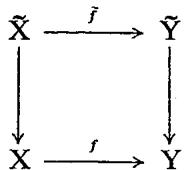
\includegraphics[keepaspectratio]{images/part001_3e847d2c.jpg}}

，并且与群 \(\{\pm1\}\) 的作用相容。

若 \(\tilde{f}\) 是 f 的一个定向，且 \(\eta\) 是 Y 的一个定向，则存在唯一一个 X 的定向 \(\xi\)，使得图表

\pandocbounded{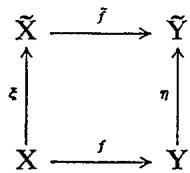
\includegraphics[keepaspectratio]{images/part001_a1f56317.jpg}}

可交换。称 \(\xi\) 由 \(\eta\) 通过 \(f\) 关联得到。

例子

\begin{enumerate}
\def\labelenumi{\alph{enumi})}
\item
  若 Y 退化为一点，则 f 的一个定向等价于 X 的一个定向。
\item
  设 \(f\) 是 étale 的。对于每个 \(x \in X\)，映射 \(\mathrm{T}_{x}(f)\) 是从 \(\mathrm{T}_{x}(\mathrm{X})\) 到 \(\mathrm{T}_{f(x)}(\mathrm{Y})\) 的同构，并通过结构转移定义一个双射
\end{enumerate}

\[
\tilde {f} _ {x}: \mathrm{Or} (\mathrm{T} _ {x} (\mathrm{X})) \rightarrow \mathrm{Or} (\mathrm{T} _ {f (x)} (\mathrm{Y})).
\]

族 \(\tilde{f}_{x}\) 定义了一个态射 \(\tilde{f}\colon\tilde{\mathbf{X}}\to\tilde{\mathbf{Y}}\)，它是 \(f\) 的一个定向，称为典范定向。

\begin{enumerate}
\def\labelenumi{\alph{enumi})}
\setcounter{enumi}{2}
\tightlist
\item
  更一般地，设 \(f\) 是浸没，并令 \(\alpha\) 为丛 T(X/Y) 的一个定向（8.1.3）。设 \(x\in X\)，且 \(\xi\) 是 \(\mathrm{T}_{x}(\mathrm{X}/\mathrm{Y})\) 的一个定向。置 \(y=f(x)\)；我们有正合序列（8.1.3）
\end{enumerate}

\[
0 \rightarrow \mathrm{T} _ {x} (\mathrm{X} / \mathrm{Y}) \rightarrow \mathrm{T} _ {x} (\mathrm{X}) \xrightarrow {\mathrm{T} _ {x} (f)} \mathrm{T} _ {y} (\mathrm{Y}) \rightarrow 0
\]

因而存在唯一一个定向 \(\tilde{f}_{\alpha}(\xi)\)，它是 \(\mathrm{T}_{y}(\mathrm{Y})\) 的定向，使得 \(\xi = \tilde{f}_{\alpha}(\xi)\alpha(x)\)（10.2.1）。映射 \(\tilde{f}_{\alpha}\colon \tilde{\mathrm{X}}\to \tilde{\mathrm{Y}}\) 是 \(f\) 的一个定向，称为与 \(\alpha\) 关联的定向。映射 \(\alpha \mapsto \tilde{f}_{\alpha}\) 是从 \(\mathrm{T}(\mathrm{X}/\mathrm{Y})\) 的定向集合到 \(f\) 的定向集合的双射。

\begin{enumerate}
\def\labelenumi{\alph{enumi})}
\setcounter{enumi}{3}
\tightlist
\item
  若 \(f: X \to Y\) 是浸入，则 \(f\) 的定向与相对于 \(f\) 的法丛的定向相对应。
\end{enumerate}

10.2.6（“乘积的定向”）。设 \(\mathbf{X}_1\)（相应地 \(\mathbf{X}_2\)）是局部有限维流形，且 \(\xi_1\)（相应地 \(\xi_2\)）是 \(\mathbf{X}_1\)（相应地 \(\mathbf{X}_2\)）的一个定向。令 \(\mathbf{X} = \mathbf{X}_1 \times \mathbf{X}_2\)。映射 \((x_1, x_2) \mapsto \xi_1(x_1)\xi_2(x_2)\)（10.2.1）是 \(\mathbf{X}_1 \times \mathbf{X}_2\) 的一个定向，称为定向 \(\xi_1\) 与 \(\xi_2\) 的乘积，记作 \(\xi_1\xi_2\) 或 \(\xi_1 \otimes \xi_2\)。

设 \(X_{i}\)（i = 1, 2）是维数为 \(n_{i}\) 的纯流形。典范同构 \(X_{1} \times X_{2} \to X_{2} \times X_{1}\) 将 \(\xi_{1} \otimes \xi_{2}\) 变为 \(\xi_{2} \otimes \xi_{1}\)（相应地变为 \(-\xi_{2} \otimes \xi_{1}\)）；若某个 \(n_{i}\) 为偶数（相应地，若 \(n_{1}\) 与 \(n_{2}\) 都为奇数）。

10.2.7（“复数情形”）。设 F 是有限维复向量空间，\(F_{R}\) 是其底层实向量空间。设 \(\{e_{1},\ldots,e_{m}\}\) 是 F 的一个基；则 \(\{e_{1},ie_{1},e_{2},ie_{2},\ldots,e_{m},ie_{m}\}\) 是 \(F_{R}\) 的一个基，而由 2m-向量定义的 \(F_{R}\) 的定向

\[
e _ {1} \wedge i e _ {1} \wedge e _ {2} \wedge i e _ {2} \wedge \dots \wedge e _ {m} \wedge i e _ {m}
\]

与 F 的基 \(\{e_{1},\ldots,e_{m}\}\) 的选取无关；这称为由给定复结构定义的 \(F_{R}\) 的定向。若 F 是两个子空间 G 与 H 的直和，则 \(F_{R}=G_{R}\oplus H_{R}\) 的定向是 \(G_{R}\) 与 \(H_{R}\) 的定向的乘积。

设 X 是一个局部有限维实流形，配备一个几乎复结构（8.8.3）。对每个 \(x \in X\)，令 \(\xi(x)\) 为其复结构定义的 \(\mathrm{T}_{x}(\mathrm{X})\) 的定向。映射 \(x \mapsto \xi(x)\) 是 X 的一个定向，称为由几乎复结构定义的定向。特别地，对于一个局部有限维复解析流形 \(X^{c}\) 的底层实解析流形 X，我们赋予它由相应几乎复结构定义的定向（8.8.6）。若把 X 上给定的复解析流形结构替换为其共轭结构（5.4.12.b)），则此定向乘以函数 \(x \mapsto (-1)^{\dim_{x} X^{c}}\)。

10.2.8. 例子

\begin{enumerate}
\def\labelenumi{\alph{enumi})}
\tightlist
\item
  设 E 是有限维实向量空间。由 E 定义的实解析流形（5.2.2）是可定向的。更确切地说，映射 \(\xi \mapsto \xi(0)\) 是从该流形的定向集合到 Or(E) 上的双射。
\end{enumerate}

特别地，流形 \(R^{n}\) 具有一个典范定向 \(\xi^{n}\)，它由半直线 \(R_{+}e_{1}\wedge\cdots\wedge e_{n}\)（属于 \(\mathrm{Or}(\mathbf{R}^{n})\)）定义。

\begin{enumerate}
\def\labelenumi{\alph{enumi})}
\setcounter{enumi}{1}
\item
  设 X 是中心为 0、半径为 \(\rho\) 的 \(\mathbf{R}^n\) 中的球面；它是 \(\mathbf{R}^n\) 的子流形。对每个 \(x \in \mathbf{X}\)，空间 \(\mathbf{T}_x(\mathbf{R}^n) = \mathbf{R}^n\) 是直线 \(\mathbf{R}x\) 与超平面 \(\mathbf{T}_x(\mathbf{X})\) 的直和。令 \(\eta_x\) 为定向 \(\mathbf{R}_+x\) 的直线 \(\mathbf{R}x\)（“向外法向”），并令 \(\xi_x\) 为 \(\mathbf{T}_x(\mathbf{X})\) 的唯一一个定向，使得 \(\eta_x\) 与 \(\xi_x\) 的乘积是定向 \(\xi^n\) 的 \(\mathbf{R}^n\)。映射 \(x \mapsto \xi_x\) 是 \(\mathbf{X}\) 的一个定向，称为典范定向。
\item
  设 X 是一个连通流形，G 是在 X 上适当地且自由地作用的离散群。X/G 可定向的充要条件是 X 可定向且 G 在 X 的定向集合上的作用是平凡的。
\item
  实射影空间 \(\mathbf{P}_{n-1}(\mathbf{R})\) 可与球面 \(S_{n-1}\) 在群 \(\{\pm1\}\) 通过 \(x\mapsto\pm x\) 的作用下的商等同；当 n 为偶数时它可定向，当 n 为奇数时它不可定向。
\item
  每个李群被连通李子群取商所得的空间都是可定向的。
\end{enumerate}

\subsection{M-扭曲微分形式}

10.3.1. 设 X 是类 \(C^{r}\) 的实流形，M 是以 X 为底空间、有限秩且类 \(C^{k}\) 的向量丛，其中 \(0 \leqslant k \leqslant r\)。令 \(\lambda_{\mathrm{M}} = (\mathrm{Or}_{\mathrm{M}}, \{\pm 1\}, \mathrm{X}, \pi)\) 为与 M 的定向流形相关的主纤维化（10.2.2）。令结构群 \(\{\pm 1\}\) 通过乘法作用于 R。我们把 \(\tilde{R}_{M}\) 记作与 \(\lambda_{M}\) 相关的、纤维类型为 R 的丛（赋予上文定义的运算律）（6.5.1）；它带有（7.10.2）一个以 X 为底、秩为 1 且类 \(C^{k}\) 的向量丛结构；称为 M-扭曲标量丛。

10.3.2. 我们有一个交换图：

\pandocbounded{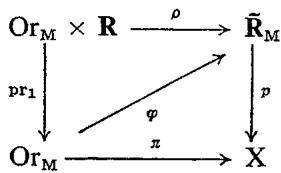
\includegraphics[keepaspectratio]{images/part001_9c73fb1b.jpg}}

其中 \(p\) 表示 \(\tilde{\mathbf{R}}_{\mathbf{M}}\) 到 \(\mathbf{X}\) 的典范投影，\(\rho\) 表示 \(\tilde{\mathbf{R}}_{\mathbf{M}}\) 的标架映射（6.5.1），并且有 \(\varphi(\xi) = \rho(\xi, 1)\)，其中 \(\xi \in \mathrm{Or}_{\mathbf{M}}\)。特别地，丛 \(\tilde{\mathbf{R}}_{\mathbf{M}}\) 在 \(\pi\) 下的逆像可与平凡丛 \(\mathrm{Or}_{\mathbf{M}} \times \mathbf{R}\) 等同。还将 \(\xi\)（\(\mathrm{Or}_{\mathbf{M}}\) 中的元素）与其在 \(\tilde{\mathbf{R}}_{\mathbf{M}}\) 中的像通过 \(\varphi\) 等同；按照这一约定，有 \(\rho(\xi, a) = a\xi\)（对所有 \((\xi, a) \in \mathrm{Or}_{\mathbf{M}} \times \mathbf{R}\)）；有 \(a\xi = b\eta\) 当且仅当存在 \(e \in \{\pm 1\}\) 使得 \(b = ea\) 且 \(\eta = e\xi\)。因此，\(\xi\) 是 \(\mathbf{M}\) 的一个定向，定义了截面 \(x \mapsto \xi(x)\)，它取值于 \(\tilde{\mathbf{R}}_{\mathbf{M}}\)。

存在唯一一个同构 \(j\)，它从 \(\tilde{\mathbf{R}}_{\mathbf{M}} \otimes \tilde{\mathbf{R}}_{\mathbf{M}}\) 到平凡丛 \(\mathbf{R}_{\mathbf{x}} = \mathbf{X} \times \mathbf{R}\)，使得 \(j(\xi \otimes \xi) = (\pi(\xi), 1)\) 对所有 \(\xi \in \mathrm{Or}_{\mathbf{M}}\) 成立；借此可将向量丛 \(\tilde{\mathbf{R}}_{\mathbf{M}}\) 与其对偶等同。

10.3.3. 设 F 还是以底空间 X 为基底、类 \(C^{r-1}\) 的向量丛。X 上取值于 \(\tilde{R}_{M} \otimes F\) 的微分形式称为取值于 F 的 M-扭曲微分形式。此类 p 次形式是丛 \(\operatorname{Alt}^{p}(\mathrm{T}(\mathrm{X}); \tilde{\mathbf{R}}_{\mathbf{M}} \otimes \mathbf{F})\) 的截面，并以显然的方式将其与 \(\tilde{R}_{M} \otimes \operatorname{Alt}^{p}(\mathrm{T}(\mathrm{X}); \mathbf{F})\) 等同。当 F 是由 Banach 空间 E 定义的平凡丛时，简称为取值于 E 的 M-扭曲形式；当 E = C（相应地 R）时，称为复 M-扭曲形式（相应地称为实 M-扭曲形式，或 M-扭曲形式）。

设 \(\omega\) 是取值于 F 的 M-扭曲形式，次数为 \(p\)。由于 \(\pi\colon\mathrm{Or}_{\mathbb{M}}\to\mathbf{X}\) 是 étale 的，且 \(\pi^{*}(\tilde{\mathbf{R}}_{\mathbb{M}})=\mathrm{Or}_{\mathbb{M}}\times\mathbf{R}\)，所以可以将 \(\pi^{*}(\tilde{\mathbf{R}}_{\mathbb{M}}\otimes\operatorname{Alt}^{p}(\mathrm{T}(\mathrm{X});\mathrm{F}))\) 与 \(\mathrm{Alt}^{p}(\mathrm{T}(\mathrm{Or}_{\mathbb{M}});\pi^{*}(\mathrm{F}))\) 等同，而 \(\omega\) 定义了 \(\tilde{\omega}\)（7.4.3）作为 \(\mathrm{Alt}^{p}(\mathrm{T}(\mathrm{Or}_{\mathbb{M}});\pi^{*}(\mathrm{F}))\) 的截面，换言之，是次数为 \(p\)、定义在 \(\mathrm{Or}_{\mathbb{M}}\) 上且取值于 \(\pi^{*}(\mathrm{F})\) 的微分形式。由此得到一个双射，从 X 上取值于 F 的 M-扭曲形式空间（次数为 \(p\)）到形式空间：其中 \(\tilde{\omega}\) 是次数为 \(p\)、定义在 \(\mathrm{Or}_{\mathbb{M}}\) 上且取值于 \(\pi^{*}(\mathrm{F})\) 的形式，且满足

\[
\tilde{\omega}(-\xi)=-\tilde{\omega}(\xi)\quad\text{对每个 }\xi\in\mathrm{Or}_{\mathbb{M}}.
\]

当 M 配备一个定向 \(\xi\) 时，映射 \(\omega \mapsto \xi \otimes \omega\) 使得可以将 \(\mathrm{Alt}^p(\mathrm{T}(\mathrm{X});\mathrm{F})\) 的截面（换言之，\(p\) 次通常微分形式）与取值于 F 的 \(p\) 次 M-扭曲形式等同。

10.3.4. 设 \(\omega\) 是 X 上取值于 Banach 空间 E、次数为 \(p\) 且类为 \(\mathbf{C}^s\) 的 M-扭曲微分形式（\(1 \leqslant s \leqslant \inf(k, r - 1)\)）。存在唯一一个 M-扭曲微分形式 \(d\omega\)，次数为 \(p + 1\)，取值于 E，且满足：对于 X 的每个开集 U、每个定向 \(\xi\)，属于 \(M|_{U}\) 的，以及 U 上的每个微分形式 \(\alpha\)，若 \(\omega|_{U} = \xi \otimes \alpha\)，则 \(d\omega|_{U} = \xi \otimes d\alpha\)。形式 \(d\omega\) 属于类 \(\mathbf{C}^{s-1}\)；称为 \(\omega\) 的外微分。

若将 \(\tilde{\omega}\)（相应地 \(\widetilde{d\omega}\)）记作 \(\mathrm{Or}_{\mathbb{M}}\) 上与 \(\omega\)（相应地与 \(d\omega\)）对应的微分形式，如 10.3.3 中那样，则有 \(d(\tilde{\omega}) = \widetilde{d\omega}\)。

若 \(\zeta\) 是类为 \(\mathbf{C}^s\) 的向量场，定义在 \(X\) 上，则以类似方式定义 M-扭曲形式 \(\theta_{\zeta}.\omega\)。有

\[
\theta_ {\zeta}. \omega = d (i (\zeta) \omega) + i (\zeta) d \omega
\]

并且 \(\theta_{\zeta}.\omega\) 属于类 \(\mathbf{C}^{s - 1}\)。

\subsection{与扭曲微分形式相关的测度}

回顾一下，在本节中，我们假定 K = R，且所考虑的所有流形都是局部有限维的。

10.4.1. 设 X 是类 \(C^{r}\) 的流形。取切丛 T(X) 作为向量丛 M，便可应用 10.3 的定义和结果。于是有 \(\mathrm{Or}_{\mathbf{M}} = \tilde{\mathbf{X}}\)（10.2.4）；我们将其记作 \(\tilde{\mathbf{R}}_{\mathbf{X}}\)，并将扭曲标量丛简单地称为丛 \(\tilde{\mathbf{R}}_{\mathrm{T}(\mathbf{X})}\)（10.3.1）\footnote{注意，当把 X 看作自身上秩为 0 的向量丛结构时，这一记号与 \(\widetilde{\mathbf{R}}_{\mathbf{M}}\) 的记号冲突。}；取值于向量丛 F 的 T(X)-扭曲微分形式简单地称为取值于 F 的扭曲（或奇）微分形式。当 X 配备一个定向时，映射 \(\omega \mapsto \xi \otimes \omega\) 使得可以将通常微分形式（有时称为“偶”微分形式）与扭曲形式等同。

10.4.2. 设 \(f\colon\mathbf{X}\to\mathbf{Y}\) 是类 \(\mathbf{C}^{r}\) 流形的态射，且 \(\tilde{f}\colon\tilde{\mathbf{X}}\to\tilde{\mathbf{Y}}\) 是 \(f\) 的一个定向（10.2.5）。存在唯一一个同构 \(j\)，从 \(f^{*}(\widetilde{\mathbf{R}}_{\mathbf{Y}})\) 到 \(\widetilde{\mathbf{R}}_{\mathbf{X}}\)，使得 \(\tilde{x}=j(\pi(\tilde{x}),\tilde{f}(\tilde{x}))\) 对所有 \(\tilde{x}\in\tilde{\mathbf{X}}\) 成立。我们通过 \(j\) 将这两个丛等同。若 \(\omega\) 是 Y 上取值于向量丛 F 的扭曲形式，次数为 \(p\)，则逆像 \(f^{*}(\omega)\) 可与 X 上次数为 \(p\)、取值于 \(f^{*}(\mathrm{F})\) 的扭曲微分形式等同。若将 \(\tilde{\omega}\)（相应地 \(\widetilde{f^{*}(\omega)}\)）记作分别位于 \(\tilde{\mathbf{Y}}\)（相应地 \(\tilde{\mathbf{X}}\)）上、与 \(\omega\)（相应地 \(f^{*}(\omega)\)）对应的微分形式，如 10.3.3 中那样，则有 \(\tilde{f}^{*}(\tilde{\omega})=\widetilde{f^{*}(\omega)}\)。

当 F 是由 Banach 空间定义的平凡丛时，运算 \(f^*\) 与外微分交换（10.3.4）。

10.4.3. 设 X 是维数为 n 的纯流形，\(\omega\) 是 X 上取值于 Banach 空间 E 的 n 次扭曲微分形式。令 \(c = (\mathrm{U}, \varphi, \mathbf{R}^{n})\) 为 X 的一个图，令 \(\xi^{n}\) 为 \(R^{n}\) 的典范定向；以 \(u^{1}, \ldots, u^{n}\) 表示 \(R^{n}\) 上的坐标函数。存在唯一一个函数 \(f_{c}\)，定义在 \(\varphi(\mathrm{U})\) 上，取值于 E，使得

\[
\omega | \mathrm{U} = \varphi^ {*} (\xi^ {n} \otimes f _ {c}. d u ^ {1} \wedge \dots \wedge d u ^ {n}).
\]

称 \(\omega\) 是局部可积的，如果对于 X 的每个图 \(c = (\mathrm{U},\varphi ,\mathbb{R}^n)\)，相应函数 \(f_{c}\) 关于 \(\lambda_{\varphi (\mathrm{U})}^{\otimes n}\) 局部可积（其中 \(\lambda\) 表示 R 上的勒贝格测度）。假定这一点成立且 X 是分离的。在 X 上存在一个取值于 E 的向量测度 \(\alpha (\omega)\)，并且唯一地具有如下性质：对于 X 的每个图 \(c = (\mathrm{U},\varphi ,\mathbb{R}^n)\)，其在 \(\varphi\) 下的像，即测度 \(\alpha (\omega)\) 在 U 上的限制，是测度 \(f_{c}\lambda_{\varphi(\mathrm{U})}^{\otimes n}\)（INT, VI, § 2, no. 4）。称 \(\alpha (\omega)\) 为由 \(\omega\) 定义的测度，并且通常仍简记为 \(\omega\)。\(\alpha (\omega)\) 的支集包含于 \(\operatorname{Supp}\omega\)（\(\omega\) 的支集）中（把微分形式 \(\omega\) 的支集定义为满足 \(x\in X\) 且 \(\omega (x)\neq 0\) 的 x 的集合的闭包）。

若 \(f\) 是 X 上关于测度 \(\alpha(\omega)\) 局部可积的实函数，则微分形式 \(f\omega\) 局部可积，且有 \(\alpha(f\omega) = f.\alpha(\omega)\)。

若 \(g\) 是 X 上关于 \(\alpha(\omega)\) 本质可积的实函数，则其积分通常记作 \(\int_{\mathbf{X}} g\omega\)、\(\int g\omega\) 或 \(\int g(x)\omega(x)\)；人们避免将其记作 \(\int g d\omega\)，因为这可能与 \(d\omega\)（\(\omega\) 的外微分）混淆；当 \(\omega\) 属于类 \(C^{1}\) 时，该外微分有定义（并且还等于 0）。若 A 是 X 的一个子集，且其示性函数 \(\varphi_{\mathrm{A}}\) 关于 \(\alpha(\omega)\) 本质可积，则 \(\varphi_{\mathrm{A}}\) 的积分记作 \(\int_{A} \omega\)。若常数 1 关于 \(\alpha(\omega)\) 本质可积，则称 \(\omega\) 是可积的。

现在令 \(p\) 为整数，满足 \(0 \leqslant p \leqslant n\)，令 \(\omega\) 为 X 上取值于 Banach 空间 E、次数为 \(p\) 的扭曲微分形式。此外，令 Y 为 X 的一个维数为 \(p\) 的纯子流形；假设典范嵌入 \(i: Y \to X\) 配备了一个定向。于是，其逆像 \(i^{*}(\omega)\)（10.4.2）有时记作 \(\omega|Y\)。若 \(\omega|Y\) 可积，置

\[
\int_ {\mathbf {Y}} \omega = \int_ {\mathbf {Y}} \omega | \mathbf {Y}.
\]

10.4.4. 设 X 是一个配备定向 \(\xi\) 的 n 维纯流形。通常微分形式与扭曲微分形式之间的等同 \(\omega \mapsto \xi \otimes \omega\) 使得可以将前述结果应用于 X 上的 n 次形式；因此，每个局部可积的 n 次形式 \(\omega\) 都关联着 X 上的一个测度，仍记作 \(\omega\)。若 E = R，则这样的形式 \(\omega\) 局部具有可积模（10.1.5），与其对应的测度 \(\text{mod}(\omega)_{\mu}\)（10.1.6）恰好是 \(|\omega|\)（测度 \(\omega\) 的绝对值）（INT, III, § 1, no. 6）。

10.4.5. 例。--- 设 X 是一个定向的、分离的 1 维纯实流形，且 \(z: \mathrm{X} \to \mathbf{C}\) 是从 X 到 C 的可微映射。复微分形式 \(dz\) 在 X 上定义了一个也记作 \(dz\) 的复测度。这尤其适用于 X 是 C 的一个 1 维纯可微子流形、\(z\) 是 X 到 C 的嵌入的情形。

更具体地，设 X 是中心为 0、半径 \(\rho > 0\) 的圆；按照 10.2.8 b) 中的指示，并利用 C 与 \(\mathbf{R}^2\) 的通常等同，为 X 赋予定向。若 \(x \in \mathbf{X}\)，切空间 \(\mathrm{T}_x(\mathbf{X})\) 可与 \(\mathbf{R}ix\) 等同，后者是 \(\mathrm{T}_x(\mathbf{C}) = \mathbf{C}\) 中的直线，而所选定向是半直线 \(\mathbf{R}_+ix\)。若 \(f\) 是 X 上取值于复 Banach 空间的连续函数，则 \(f\) 关于测度 \(dz\) 的积分由公式给出

\[
\int_ {\mathbb {X}} f (z) d z = i \rho \int_ {0} ^ {2 \pi} f (\rho e ^ {i \alpha}) e ^ {i \alpha} d \alpha .
\]

例如，若 \(n\) 是一个整数，则有

\[
\int_ {\mathrm{X}} z ^ {n} d z = i \rho^ {n + 1} \int_ {0} ^ {2 \pi} e ^ {(n + 1) i \alpha} d \alpha = \left\{ \begin{array}{l l} 0 & \quad \text {if } n \neq - 1 \\ 2 i \pi & \quad \text {if } n = - 1. \end{array} \right.
\]

10.4.6（“复数情形”）。设 \(X^{c}\) 是一个分离的、纯维数为 \(m\) 的复解析流形，且 \(\omega\) 是次数为 \(m\) 的全纯微分形式，定义在 \(X^{c}\) 上。设 X 是 \(X^{c}\) 的底层实解析流形；形式 \(\omega\) 与 X 上的 \((m,0)\) 型形式等同（8.8.9）；令 \(\overline{\omega}\) 为其共轭（8.8.2）。形式 \(i^{m^{2}}\omega \wedge \overline{\omega}\) 是 X 上次数为 \(2m\) 的实微分形式；考虑到 X 的典范定向（10.2.7），此形式与 X 上的一个测度等同，而该测度正是 10.1.6 中定义的正测度 \(\operatorname{mod}(\omega)_{\mu}\)，其中 \(\mu\) 是由微分形式 \(i \, dz \wedge \overline{dz}\) 定义的测度，换言之，是测度 \(\lambda^{\otimes 2}\) 在 \(\mathbf{C}\) 上的两倍（按通常方式与 \(\mathbf{R}^{2}\) 等同）。

令 H 为由全纯形式 \(\omega\)（次数为 \(m\)，定义在 \(\mathbf{X}^c\) 上）组成的空间，使得测度 \(\omega \wedge \overline{\omega}\) 有界。对于 H 中的 \(\alpha, \beta\)，复测度 \(\alpha \wedge \overline{\beta}\) 有界；令

\[
(\alpha | \beta) = i ^ {m ^ {2}} \int_ {\mathbf {X}} \alpha \wedge \bar {\beta},
\]

从而得到 H 上的一个厄米形式，它使 H 成为 Hilbert 空间。

\section{Stokes 公式}

本段中，我们假定 K = R。

\subsection{片段}

11.1.1. 设 E 是 Banach 空间。如果存在连续线性泛函 \(h \neq 0\) 和实数 k 使得 \(S = \{x|h(x) \leqslant k\}\)，则 E 的子集 S 称为闭半空间（参见 EVT, II, §2, no. 6）；此时 S 的边界是闭超平面 \(\{x|h(x) = k\}\)；它也称为 S 的边界，记作 \(\partial S\)。

11.1.2. 设 X 是类 \(C^{r}\) 流形，A 是 X 的一个子集。如果对每个 \(a \in A\)，都存在 X 在 a 处的图 \(c = (U, \varphi, E)\)，使得 \(\varphi(A \cap U)\) 是 E 的某个闭半空间的开子集，则称 A 是 X 的一个片段。置 \(\partial A = A - \mathring{A}\)（A 的非内部点的集合）。它是 A 的子流形，称为 A 的边界。\footnote{这一术语源于以下事实：A 自然地带有一个“带边界的流形”结构，其边界为 \(\partial A\)。关于这一范畴的定义，以及更一般的“带角流形”范畴，读者可参阅 H. Cartan, \emph{Séminaire 1961/62, Topologie Différentielle}, lectures 1–2–3（A. Douady），Benjamin, New York, 1969。需要指出的是，可以证明，每个边界为仿紧的“带边界流形”都同构于某个流形的闭片段。}若 \(a \in \partial A\)，则存在 X 在 a 处、以 a 为中心的图 \(c = (U, \varphi, E)\) 以及 E 的闭超平面 H，使得 \(\varphi(A \cap U)\) 是由 H 定义的 E 的某个闭半空间 \(S_{c}\) 中 0 的一个开邻域（EVT, II, § 2, no. 6），并且 \(\varphi(\partial A \cap U) = H \cap \varphi(A \cap U)\)。这样的图称为 A 在 a 处的适配图。于是，闭半空间 \(S_{c}\) 是使 \(\varphi(A \cap U)\) 成为开集的唯一 E 的闭半空间。

对于 X 的一个闭子集 A，它成为 X 的片段的充要条件是：\(\mathring{A}\) 在 A 中稠密，并且 \(A-\mathring{A}\) 在其每一点处都是 X 的余维 1 子流形。

11.1.3. 例子

\begin{enumerate}
\def\labelenumi{\alph{enumi})}
\item
  在 \(\mathbf{R}^{n}\) 中，半径 \(>0\) 的闭球是一个片段；其边界是相应的球面。
\item
  若 A 是流形 X 的一个片段，且 B 是 \(\partial A\) 的闭子集，则 A - B 是 X 的一个片段。
\item
  设 \(\varphi: X \to X'\) 是类 \(C^r\) 的流形态射，且 \(A'\) 是 \(X'\) 的一个片段。若 \(\varphi\) 与 \(\partial A'\) 横截（5.11.6），则 \(\varphi^{-1}(A')\) 是 \(X\) 的一个片段，其边界为 \(\varphi^{-1}(\partial A')\)。
\end{enumerate}

特别地，设 \(h: \mathbf{X} \to \mathbf{R}\) 是类 \(\mathbf{C}^r\) 的函数，且 \(a \in \mathbf{R}\)；假定不存在 \(x \in \mathbf{X}\) 使得 \(h(x) = a\) 且 \(d_x h = 0\)。集合 \(\{x | h(x) \leqslant a\}\) 是 \(\mathbf{X}\) 的一个闭片段，其边界为 \(h^{-1}(a)\)。

\begin{enumerate}
\def\labelenumi{\alph{enumi})}
\setcounter{enumi}{3}
\tightlist
\item
  若 \(r = \infty\) 且 X 局部紧，则 X 的每个紧子集都有一个由紧片段组成的邻域基本系。
\end{enumerate}

11.1.4. 设 X 是类 \(\mathbf{C}^{\mathrm{r}}\) 的流形，A 是 X 的一个片段。设 \(a \in \partial \mathrm{A}\)，\(v \in \mathrm{T}_a(\mathrm{X})\)。令 \(c = (\mathrm{U}, \varphi, \mathrm{E})\) 为 A 在 \(a\) 处的适配图（11.1.2），并令 \(h = \theta_c^{-1}(v)\) 为 E 中与 \(v\) 对应的元素（5.5.1）。令 \(\mathrm{S}_c\) 为 E 的闭半空间，使得 \(\varphi(\mathrm{A} \cap \mathrm{U})\) 是其开子集（11.1.2）。称 \(v\) 是 A 在 \(a\) 处的向内（相应地严格向内、向外、严格向外）向量，当且仅当 \(h\) 属于 \(\mathrm{S}_c\)（相应地属于 \(\dot{\mathrm{S}}_c\)、\(-\mathrm{S}_c\)、\(-\dot{\mathrm{S}}_c\)）；这个条件与适配图 \(c\) 的选择无关。我们把 \(\mathrm{T}_a^+(\mathrm{A})\)（相应地 \(\mathrm{T}_a^-(\mathrm{A})\)）记作 A 的向外（相应地向内）向量在 \(\mathrm{T}_a(\mathrm{X})\) 中的集合。这些是 \(\mathrm{T}_a(\mathrm{X})\) 的闭半空间，其边界包含 0。于是有

\[
\mathrm{T} _ {a} (\partial \mathrm{A}) = \mathrm{T} _ {a} ^ {+} (\mathrm{A}) \cap \mathrm{T} _ {a} ^ {-} (\mathrm{A}).
\]

\subsection{片段的 Stokes 公式}

本节中，X 表示类 \(C^{r}\)（\(r \geqslant 2\)）的纯有限维分离流形。A 表示 X 的一个片段，i 表示将 \(\partial A\) 典范嵌入 X 的映射。E 表示 Banach 空间。

11.2.1. 设 \(x \in \partial A\)，且 \(\xi\) 是 \(T_x(\partial A)\) 的一个定向；把 \(\tilde{i}_x(\xi)\) 记作 \(T_x(X)\) 的一个定向，其中含有元素 \(v \wedge u\)，这里 \(v\) 是 A 在 x 处的严格向外向量（11.1.4），而 \(u\) 是 \(\bigwedge^{n-1} T_x(\partial A)\) 中属于定向 \(\xi\) 的非零元素。映射 \(\tilde{i}_x\) 是从 \(\text{Or}(T_x(\partial A))\) 到 \(\text{Or}(T_x(X))\) 的双射。对于映射 \(\tilde{i}_x\)（\(x \in \partial A\)），它定义了一个态射 \(\tilde{i} \colon \partial \widetilde{A} \to \widetilde{X}\)，它是 \(i\) 的一个定向（10.2.5）。若 \(\xi\) 是 X 的一个定向，则 \(\partial A\) 的定向与 \(\xi\) 相关联，并由 \(\tilde{i}\) 得到（10.2.5），称为由 \(\xi\) 定义的定向。

例。--- 当 \(X = R^{n}\) 时，\(\xi\) 是 \(R^{n}\) 的通常定向，且 A 是半径 \(\rho>0\) 的闭球；球面 \(\partial A\) 的定向由 \(\xi\) 定义，就是典范定向（10.2.8, b)）。

11.2.2. 设 \(\omega\) 是 X 上取值于 Banach 空间 E 的 \(p\) 次扭曲微分形式（10.4.1）；其逆像 \(i^{*}(\omega)\) 是 \(\omega\) 通过有向态射 \(i\colon\partial A\to X\) 得到的逆像，记作 \(\omega|\partial A\)，称为 \(\omega\) 在 \(\partial A\) 上诱导的形式（参见 10.4.3）。

11.2.3. 我们作如下两个假设之一：

\begin{enumerate}
\def\labelenumi{(\roman{enumi})}
\tightlist
\item
  \(\omega\) 是 X 上取值于 E 的 \(n - 1\) 次扭曲微分形式；
\item
  X 是有向的，\(\partial A\) 配备与之相应的定向（11.2.1），且 \(\omega\) 是 X 上取值于 E 的 \(n - 1\) 次微分形式。
\end{enumerate}

进一步假设 \(\omega\) 属于类 \(C^{1}\)，且 A 与 \(\omega\) 的支集的交是紧的。\(d\omega\) 是 \(\omega\) 的外微分，并且连续（8.3.5 和 10.3.4）。

A 的示性函数关于 X 上由 \(d\omega\) 定义的向量测度是本质可积的，而 \(\omega|\partial\mathrm{A}\) 是 \(n-1\) 次定义在 \(\partial\mathrm{A}\) 上的微分形式，并且可积（10.4.3 和 10.4.4）。有

\[
\int_ {\mathrm{A}} d \omega = \int_ {\partial \mathrm{A}} \omega \quad (\text{Stokes公式})
\]

11.2.4. 设 \(\alpha\) 是 X 上取值于 Banach 空间 E、具有紧支集、次数为 \(n\) 且类为 \(\mathbf{C}^1\) 的扭曲微分形式。若存在 X 上取值于 E、具有紧支集的扭曲微分形式 \(\omega\)，其次数为 \(n - 1\) 且类为 \(\mathbf{C}^1\)，使得 \(\alpha = d\omega\)，则必须有 \(\int_{\mathbb{X}} \alpha = 0\)。若 X 连通，则此条件充分；此外，若 \(\alpha\) 属于类 \(\mathbf{C}^k\)（\(k\leqslant r-1,\ k\neq\omega\)），则可以选取 \(\omega\) 为类 \(\mathbf{C}^k\)。

11.2.5. 假设 X 是 \(\mathbf{C}\) 的底层实流形，E 是复 Banach 空间，A 是 X 的一个紧片段。赋予 X 由其复结构定义的定向（10.2.7）。设 f 是从 A 到 E 的连续映射，且其在 A 的内部 \(\mathring{A}\) 上的限制是全纯的。以 \(dz\) 表示嵌入 \(z\colon\partial A\to\mathbf{C}\) 的微分。形式 \(f\cdot dz\)，即 f 与 dz 的乘积，是 \(\partial A\) 上取值于 E 的 1 次微分形式，属于类 \(C^{0}\)，并且有：

\[
\int_ {\partial \mathbf {A}} f\, d z = 0 \quad (\text{Cauchy公式})
\]

当 \(f\) 可延拓为定义在 A 的某个开邻域 U 上、仍记作 \(f\) 的全纯映射时，形式 \(f.dz\)（此时 z 表示 U 到 \(\mathbf{C}\) 的典范嵌入）在 U 上属于类 \(C^{\omega}\)，且其外微分为零。

11.2.6（“积分的导数”）。假设 X 是有向的。设 Y 是类 \(C^{r}\) 的流形，\(\alpha\) 是 Y 上取值于 E、具有紧支集、次数为 \(n\)、类为 \(C^{1}\) 的微分形式。设 I 是包含 0 的 R 的开子集，\(g: I \times X \to Y\) 是类 \(C^{r}\) 的态射；对于 \(t \in I\)，记 \(g_{t}\) 为从 X 到 Y 的映射 \(x \mapsto g(t, x)\)。令 \(\psi\) 为从 X 到 T(Y) 的态射，由 \(\psi(x) = T_{(0,x)}(g)(1,0)\) 定义；它是 \(g_{0}\) 的一个提升（8.6.5）。假设 \(\operatorname{pr}_{1}\colon I\times A\to I\) 限制在 \(I\times A\) 与 \(g^{*}(\alpha)\) 的支集的交集上是本原的（TG, I, § 10）。则对于每个 \(t \in I\)，A 与 \(g_{t}^{*}(\alpha)\) 的支集的交是紧的；映射 \(t \mapsto \int_{A} g_{t}^{*}(\alpha)\) 在 I 上属于类 \(C^{1}\)，且其在原点处的导数由公式给出

\[
\frac {d}{d t} \left(\int_ {\mathrm{A}} g _ {t} ^ {*} (\alpha)\right) _ {t = 0} = \int_ {\mathrm{A}} \theta_ {\psi}. \alpha = \int_ {\mathrm{A}} i (\psi) d \alpha + \int_ {\partial \mathrm{A}} i (\psi) \alpha ,
\]

参见第 8.6 号。

\subsection{局部多面体集的 Stokes 公式}

本号中，X 表示类 \(C^{r}\)（\(r \geqslant 2\)）的有限维纯实流形；我们假定 X 是分离的。\footnote{读者若对更一般的情形感兴趣，可参阅 H. Whitney, \emph{Geometric Integration Theory}, 第 III 章 § 18（Princeton Univ. Press, 1957）。}

11.3.1. 设 A 是有限维实向量空间的一个子集。如果 A 是有限个闭半空间的有限交的并，则称 A 是多面体的。

称 X 的子集 A 是局部多面体的，如果对于每个 \(x \in X\)，都存在 X 在 x 处的图 \(c = (\mathrm{U}, \varphi, \mathrm{E})\) 以及 E 的一个多面体子集 \(A_{c}\)，使得 \(\varphi(\mathrm{A} \cap \mathrm{U}) = \varphi(\mathrm{U}) \cap \mathrm{A}_{c}\)。X 的一个片段是局部多面体子集。

11.3.2. 设 A 是 X 的闭子集，令 \(\mathrm{Fr}(\mathrm{A}) = \mathrm{A} - \mathring{\mathrm{A}}\) 为其边界。称 \(x \in \mathrm{Fr}(\mathrm{A})\) 为正则点，如果存在 x 的一个开邻域 U，使得 \(A \cap U\) 是流形 U 的一个片段（此时 x 属于 \(A \cap U\) 的边界）。我们把 \(\partial A\) 记作 \(\mathrm{Fr}(\mathrm{A})\) 的正则点集合，并称其为 A 的正则边界（或简称边界）。集合 \(A' = \mathring{A} \cup \partial A\) 是 X 的一个片段，其边界为 \(\partial A\)。

11.3.3. * 例。--- 设 \(\mathcal{H}\) 是维数为 \(n\) 的有限维实仿射空间 E 中的一个局部有限超平面集，C 是相对于 \(\mathcal{H}\) 的 E 的一个室（LIE, V, § 1, no. 3）。C 的闭包 \(\overline{\mathbf{C}}\) 是流形 E 的局部多面体子集；\(\overline{\mathbf{C}}\) 的正则边界是 C 的各个面的并（同上，no. 4）。特别地，若 C 是一个开单纯形（同上，no. 6），顶点为 \(a_0, \ldots, a_n\)，则 \(\overline{\mathbf{C}}\) 的边界是各个 \(\overline{\mathbf{C}_{\{i\}}}\)（\(0 \leqslant i \leqslant n\)）的并，其中 \(\mathbf{C}_{\{i\}}\) 是由顶点 \(a_0, \ldots, a_{i-1}, a_{i+1}, \ldots, a_n\) 在这些顶点生成的仿射空间中的开单纯形。*
11.3.4. 设 A 是 X 的局部多面体子集，\(\omega\) 是 X 上取值于 Banach 空间 E 的 \(n - 1\) 次扭曲微分形式；假设 \(\omega\) 属于类 \(\mathbf{C}^1\)，且其支集与 A 的交是紧的。于是，A（相应地 \(A'\)、\(\mathring{A}\)）的示性函数关于 X 上由 \(d\omega\) 定义的向量测度都是本质可积的，并且有

\[
\int_ {\mathrm{A}} d \omega = \int_ {\mathrm{A} ^ {\prime}} d \omega = \int_ {\mathring{\mathrm{A}}} d \omega.
\]

形式 \(\omega|\partial\mathbf{A}\)（对于 \(\partial\mathbf{A}\) 的典范嵌入所带的典范定向，该嵌入被看作片段 \(\mathbf{A}'\) 的边界并嵌入 \(\mathbf{X}\)）在 \(\partial\mathbf{A}\) 上可积，并且有

\[
\int_ {\mathbf {A}} d \omega = \int_ {\partial \mathbf {A}} \omega \quad (\text{Stokes公式}).
\]

当 X 配备一个定向、\(\partial\mathbf{A}\) 配备相应的定向（11.2.1）时，如果 \(\omega\) 是 X 上取值于 E 的 \(n-1\) 次普通微分形式、属于类 \(\mathbf{C}^{1}\)，且 \(\mathbf{A}\cap\operatorname{Supp}\omega\) 是紧的，则此公式仍然成立。

\subsection{相对 Stokes 公式（沿纤维积分）}

本号中，X 和 S 表示两个类 \(C^{r}\) 的（实）流形，且 \(\pi: X \to S\) 是一个浸没。我们记 n 为一个整数，并假定对于每个 \(s \in S\)，纤维 \(X_{s} = \pi^{-1}(s)\) 是 \(\pi\) 在 s 处的纤维（它是 X 的子流形（5.10.5）），都是纯 n 维的。

11.4.1. 设 E 和 H 是两个向量空间，F 是 H 的一个 n 维有限维向量子空间。

令 p 为一个满足 \(\geqslant0\) 的整数，令 u 为一个交错的 \((n+p)\)-线性映射，从 \(H^{n+p}\) 到 E，令 \(t_{1},\ldots,t_{p}\) 为 \(H/F\) 的元素；令 \(t_{1}^{\prime},\ldots,t_{p}^{\prime}\) 为 \(t_{1},\ldots,t_{p}\) 在 H 中的代表元。映射

\[
(x _ {1}, \dots , x _ {n}) \mapsto u (t _ {1} ^ {\prime}, \dots , t _ {p} ^ {\prime}, x _ {1}, \dots , x _ {n})
\]

是从 \(\mathbf{F}^n\) 到 E 的 n-线性交错映射，它只依赖于 u 和 \(t_i\)；记作 \(u \perp (t_1, \ldots, t_p)\)（对于特殊情形 \(\mathbf{E} = \mathbf{K}\)，参见 A, III, p. 158）。映射

\[
\left(t _ {1}, \dots , t _ {p}\right) \mapsto u \perp \left(t _ {1}, \dots , t _ {p}\right)
\]

是 p-线性交错的。

11.4.2（“\(\pi\)-扭曲”）。考虑 X 上的向量丛 \(\mathrm{T}(\mathrm{X}/\mathrm{S})\)（8.1.3）；它在 X 的每一点处都有有限秩 n。置 \(\tilde{R}_{\pi} = \tilde{R}_{T(X/S)}\)（10.3.1），\(\tilde{X}_{\pi} = \mathrm{Or}_{T(X/S)}\)（10.2.2）。设 \(s \in S\)；利用 \(\mathrm{T}(\mathrm{X}/\mathrm{S})|_{\mathbf{X}_{s}}\) 与 \(\mathrm{T}(\mathbf{X}_{s})\) 的自然等同（8.1.3），复合映射 \(\tilde{\pi}: \tilde{X}_{\pi} \to S\)（它是 \(\pi\) 与典范映射 \(\tilde{X}_{\pi} \to X\) 的复合）在 s 处的纤维是 \(\tilde{X}_{s}\)（10.2.4）。X 上的 \(\pi\)-扭曲微分形式称为 \(\mathrm{T}(\mathrm{X}/\mathrm{S})\)-扭曲微分形式（10.3.3）。

11.4.3（“S-态射的 S-定向”）。设 \(\mathbf{X}'\) 是一个配备浸没 \(\pi'\colon\mathbf{X}'\to\mathbf{S}\) 的簇，其纤维 \(\mathbf{X}'_{s}\) 都是纯有限维 \(n'\) 维的；设 \(\varphi\colon\mathbf{X}'\to\mathbf{X}\) 是满足 \(\pi'=\pi\circ\varphi\) 的态射。一个 \(\varphi\) 的 S-定向是态射 \(\tilde{\varphi}\colon\tilde{\mathbf{X}}'_{\pi'}\to\tilde{\mathbf{X}}_{\pi}\)，它与群 \(\{\pm1\}\) 的作用交换，并使图表可交换。

\pandocbounded{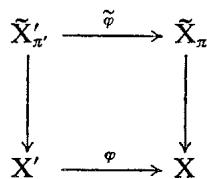
\includegraphics[keepaspectratio]{images/part001_c0391fc0.jpg}}

为 \(\varphi\) 配备 S-定向的数据使得可以像在 10.4.2 中那样，将丛 \(\tilde{\mathbf{R}}_{\pi'}\) 与 \(\varphi^{*}(\tilde{\mathbf{R}}_{\pi})\) 等同，并定义对 \(\pi\)-扭曲微分形式通过 S-定向态射 \(\varphi\) 的拉回；它是 \(\pi'\)-扭曲微分形式，定义在 \(\mathbf{X}'\) 上。

11.4.4. 设 A 是 X 的一个片段，使得 \(\pi\) 在 \(\partial\mathbf{A}\) 上的限制是浸没。对每个 \(s\in\mathbf{S}\)，纤维 \(\mathbf{X}_{s}=\pi^{-1}(s)\) 是与 \(\partial\mathbf{A}\) 横截的 X 的子流形，而 \(\mathbf{A}\cap\mathbf{X}_{s}\) 是 \(\mathbf{X}_{s}\) 的一个片段，记作 \(\mathbf{A}_{s}\)，其边界为 \(\partial\mathbf{A}\cap\mathbf{X}_{s}\)。

令 \(i\) 为将 \(\partial\mathbf{A}\) 典范嵌入 X 的映射。存在唯一一个 S-定向 \(\tilde{i}\)，它是 \(i\) 的定向，使得对于每个 \(s\in\mathbf{S}\)，\(\tilde{i}\) 在 \((\partial\mathbf{A}_{s})^{\sim}\) 上的限制（将其与浸没 \(\partial\widetilde{\mathbf{A}}_{\pi|\partial\mathbf{A}}\to\mathbf{S}\) 在 s 处的纤维等同）是 11.2.1 中定义的、将 \(\partial\mathbf{A}_{s}\) 典范嵌入 \(\mathbf{X}_{s}\) 的映射的定向。若 \(\omega\) 是 X 上的 \(\pi\)-扭曲微分形式，则 \(\omega\) 通过上述带定向的态射 \(i\) 得到的逆像记作 \(\omega|\partial\mathbf{A}\)（参见 11.2.2）。

11.4.5（“内插积”）。令 p 为满足 \(\geqslant 0\) 的整数，令 \(\omega\) 为 X 上取值于以 X 为底空间的向量丛 E 的 \(\pi\)-扭曲微分形式，次数为 \(n + p\)。设 \(s \in S\)，\(x \in X_s\)；有 \(\omega(x) = \xi \otimes u\)，其中 \(\xi\) 是 \(T_x(X_s) = T(X/S)_x\) 的定向，与 \((\tilde{\mathbf{R}}_{X_s})_x = (\tilde{\mathbf{R}}_n)_x\) 中的元素等同（10.3.2），而 u 是一个交错 \((n + p)\)-线性映射，从 \(T_x(X)\) 到 \(E_x\)。令 \(t_1, \ldots, t_p\) 为 s 处 S 的切向量。置

\[
\theta (x) = \xi \otimes (u \llcorner (t _ {1}, \dots , t _ {p})) \in (\tilde {\mathbf {R}} _ {\mathrm{X} _ {s}}) _ {x} \otimes (\mathrm{Alt} ^ {n} (\mathrm{T} (\mathrm{X}); \mathrm{E})) _ {x}
\]

（参见 11.4.1）。于是得到 \(\theta: x \mapsto \theta(x)\)，它是 \(X_s\) 上的一个次数为 n 的扭曲微分形式，取值于 \(E|_{X_{s}}\)。将其记作 \(\omega \perp (t_1, \ldots, t_p)\)。

特别地，设 M 是以 S 为底空间、类 \(C^{r-1}\) 的向量丛，并取 \(E = \pi^{*}(M)\)。丛 \(E|_{X_{s}}\) 自然地可与以 \(X_{s}\) 为底、由 Banach 空间 \(M_{s}\) 定义的平凡丛等同，而形式 \(\omega\perp(t_{1},\ldots,t_{p})\) 可与 \(X_{s}\) 上取值于 \(M_{s}\) 的扭曲微分形式等同。

11.4.6. 保留前述记号（特别是 \(E=\pi^{*}(M)\)），并进一步假定 X 是分离的且 \(\omega\) 是连续的。设 A 是 X 的一个片段，使得 \(\pi\) 在 \(\partial A\) 上的限制是浸没，且 \(\pi\) 在 A 与 \(\omega\) 的支集的交上的限制是本原的。对于 \(s \in S\) 和 \(t_{1},\ldots,t_{p}\in\mathrm{T}_{s}(\mathrm{S})\)，形式 \(\omega \perp (t_{1}, \ldots, t_{p})\)（11.4.5）是 \(X_{s}\) 上连续的 n 次扭曲微分形式，取值于 Banach 空间 \(M_{s}\)，并且其支集与 \(A_{s}\) 的交是紧的。存在唯一一个 S 上取值于向量丛 M 的 p 次微分形式 \(\alpha\)，使得

\[
\alpha (s) \left(t _ {1}, \dots , t _ {p}\right) = \int_ {\mathrm{A} _ {s}} \omega \perp \left(t _ {1}, \dots , t _ {p}\right)
\]

对于所有 \(s \in S\) 和 \(t_{1},\ldots,t_{p}\in\mathrm{T}_{s}(\mathrm{S})\) 都成立。形式 \(\alpha\) 记作 \(\int_{\pi|\mathbf{A}} \omega\)（或简记为 \(\int_{\pi} \omega\)，当 \(\mathbf{A} = \mathbf{X}\) 时）；称它为对 \(\omega\) 在 \(\mathbf{A}\) 上沿 \(\pi\) 的纤维积分所得的形式。若 \(\omega\) 属于类 \(\mathbf{C}^{k}\)（\(0\leqslant k\leqslant r-1,\ k\leqslant\omega\)），则 \(\int_{\pi|\mathbf{A}} \omega\) 也属于同一类。

当 \(\omega\) 是次数 \(< n\) 的形式时，约定 \(\int_{\pi|\mathbf{A}} \omega = 0\)。

11.4.7. 保留前述假设和记号。

\begin{enumerate}
\def\labelenumi{\alph{enumi})}
\tightlist
\item
  对于 S 上的每个连续标量微分形式 \(\beta\)，有
\end{enumerate}

\[
\int_ {\pi | \mathrm{A}} (\pi^ {*} \beta) \wedge \omega = \beta \wedge \int_ {\pi | \mathrm{A}} \omega .
\]

\begin{enumerate}
\def\labelenumi{\alph{enumi})}
\setcounter{enumi}{1}
\tightlist
\item
  令 \(\eta\) 是 X 上的连续向量场，\(\zeta\) 是 S 上的连续向量场，并且 \(\eta\) 关于 \(\pi\) 与 \(\zeta\) 相关（8.2.6）。有
\end{enumerate}

\[
i (\zeta) \int_ {\pi | \mathrm{A}} \omega = \int_ {\pi | \mathrm{A}} i (\eta) \omega .
\]

\begin{enumerate}
\def\labelenumi{\alph{enumi})}
\setcounter{enumi}{2}
\tightlist
\item
  进一步假设 \(\eta\)、\(\zeta\) 和 \(\omega\) 属于类 \(\mathbf{C}^1\)，且有 \(\eta(x) \in \mathrm{T}_x(\partial \mathbf{A})\) 对所有 \(x \in \partial \mathbf{A}\) 成立，并且 \(\mathbf{M}\) 是由 Banach 空间 E 定义的平凡丛。我们有
\end{enumerate}

\[
\theta_ {\zeta}. \int_ {\pi | \mathrm{A}} \omega = \int_ {\pi | \mathrm{A}} \theta_ {\eta}. \omega ,
\]

（参见 8.4.2 和 10.3.4）。

\begin{enumerate}
\def\labelenumi{\alph{enumi})}
\setcounter{enumi}{3}
\tightlist
\item
  若 \(\omega\) 的次数为 \(n + p\) 且属于类 \(\mathbf{C}^1\)，则有
\end{enumerate}

\[
d \left(\int_ {\pi | \mathrm{A}} \omega\right) = \int_ {\pi | \mathrm{A}} d \omega + (- 1) ^ {p} \int_ {\pi | \partial \mathrm{A}} \omega | \partial \mathrm{A}.
\]

\begin{enumerate}
\def\labelenumi{\alph{enumi})}
\setcounter{enumi}{4}
\tightlist
\item
  假设 S 退化为一点。此时 X 上的 \(\pi\)-扭曲形式就是通常的扭曲形式（10.4.1）。若 \(\omega\) 的次数为 \(n\)，则 S 上的 0 次形式 \(\int_{\pi|A} \omega\) 是常数 \(\int_{A} \omega\)（10.4.3）。
\end{enumerate}

11.4.8. 设 \(\pi': S \to S'\) 是一个浸没；其 \(\pi'\) 的纤维是维数恒定且有限的纯 \(n'\) 维子流形。置 \(\pi'' = \pi' \circ \pi\)；它是 X 到 \(S'\) 的一个浸没，其纤维是维数 \(m = n + n'\) 的纯子流形。

设 \(x\in X\)。序列

\[
0 \longrightarrow \mathrm{T} (\mathrm{X} / \mathrm{S}) _ {x} \stackrel {\mathrm{Id}} {\longrightarrow} \mathrm{T} (\mathrm{X} / \mathrm{S} ^ {\prime}) _ {x} \stackrel {\mathrm{T} _ {x} (\pi)} {\longrightarrow} \mathrm{T} (\mathrm{S} / \mathrm{S} ^ {\prime}) _ {\pi (x)} \longrightarrow 0
\]

是正合的。存在唯一一个同构 \(j\)，它从向量丛 \(\tilde{\mathbf{R}}_{\pi} \otimes \pi^{*}(\tilde{\mathbf{R}}_{\pi'})\) 到 \(\tilde{\mathbf{R}}_{\pi'}\)，使得若 \(\xi\)（相应地 \(\eta\)）是 \(\mathrm{T}(\mathrm{X}/\mathrm{S})_x\)（相应地 \((\pi^{*}\mathrm{T}(\mathrm{S}/\mathrm{S}'))_x\)，将其与 \(\mathrm{T}(\mathrm{S}/\mathrm{S}')_{\pi(x)})\) 等同）的一个定向，则 \(j(\xi \otimes \eta) = \eta\xi\)（乘积由前述正合序列（10.2.1）定义）。

令 M' 是以 S' 为底空间的向量丛；置 \(\mathbf{M} = \pi'^{*}(\mathbf{M}')\)，且 \(\mathbf{E}=\pi^{*}(\mathbf{M})=\pi''^{*}(\mathbf{M}')\)。若 \(\omega\) 是 X 上取值于 E 的 \(\pi''\)-扭曲微分形式，则利用同构 j，可将其与一个 \(\pi\)-扭曲形式等同，该形式取值于 \(\pi^{*}(\tilde{\mathbf{R}}_{\pi'}) \otimes \mathbf{E}\)，或等价地，与取值于 \(\pi^{*}(\tilde{\mathbf{R}}_{\pi'} \otimes \mathbf{M})\) 的形式等同。

再设 A 是 X 的一个片段，使得 \(\pi|\partial\mathrm{A}:\partial\mathrm{A}\to\mathrm{S}\) 是浸没；于是 \(\pi''|\partial\mathrm{A}:\partial\mathrm{A}\to\mathrm{S}'\) 也如此。进一步假设 \(\omega\) 连续，且 \(\pi''\) 在 \(\mathbf{A}\cap\operatorname{Supp}\omega\) 上的限制是本原的；则 \(\pi\) 在 \(\mathbf{A}\cap\operatorname{Supp}\omega\) 上的限制也如此。一方面，可以考虑微分形式 \(\int_{\pi''|\mathrm{A}}\omega\) 在 \(\mathrm{S}'\) 上，它取值于 \(\mathrm{M}'\)；另一方面，可以考虑微分形式 \(\int_{\pi|\mathrm{A}}\omega\) 在 \(\mathrm{S}\) 上，它是取值于 \(\tilde{\mathbf{R}}_{\pi'}\otimes\mathrm{M}\) 的形式，或等价地，是一个 \(\pi'\)-扭曲形式，取值于 \(\mathbf{M}=\pi'^{*}(\mathbf{M}')\)。此外，\(\pi(\mathrm{A})\) 是 \(\mathrm{S}\) 的一个开子流形，且 \(\pi'\) 在 \(\pi(\mathrm{A})\cap\mathrm{Supp}\int_{\pi|\mathrm{A}}\omega\) 上的限制是本原的。形式 \(\int_{\pi'|\pi(\mathrm{A})}\int_{\pi|\mathrm{A}}\omega\) 有定义；它是 \(\mathrm{S}'\) 上取值于 \(\mathrm{M}'\) 的微分形式。有

\[
\int_ {\pi^ {\prime} \circ \pi | A} \omega = \int_ {\pi^ {\prime} | \pi (A)} \int_ {\pi | A} \omega .
\]

若 A = X，则有

\[
\int_ {\pi^ {\prime} \circ \pi} \omega = \int_ {\pi^ {\prime}} \int_ {\pi} \omega .
\]

\section{喷射}

本段中，X 和 Y 表示类 \(\mathbf{C}^r\) 的两个流形，其中 \(r \in \mathbb{N}_{\mathbb{K}}\)，并令 \(k\) 为满足 \(0 \leqslant k \leqslant r\) 的整数。

从第 12.3 号起，我们假定：

或者 K 的特征为零；

或者，所考虑的流形、Banach 空间和向量丛都是局部有限维的。

\subsection{映射的喷射}

12.1.1. 设 \(x \in X\)，且 \(f, g\) 是在 \(x\) 的邻域内定义、取值于 \(Y\) 的两个连续映射。我们称 \(f\) 与 \(g\) 有阶数 \(\geqslant k\) 的接触于 \(x\) 处，是指 \(f(x) = g(x)\)，并且存在图表 \((U, \varphi, E)\)，它是 \(X\) 在 \(x\) 处的图表，以及图表 \((V, \psi, F)\)，它是 \(Y\) 在 \(f(x)\) 处的图表，使得映射 \(\psi \circ f \circ \varphi^{-1}\) 和 \(\psi \circ g \circ \varphi^{-1}\) 在 \(\varphi(x)\) 处有阶数 \(\geqslant k\) 的接触，并且在 E 中 \(\varphi(x)\) 的某邻域内定义、取值于 F。（1.1.2）。于是，这一性质对 \(X\) 在 \(x\) 处的所有图表以及 \(Y\) 在 \(f(x)\) 处的所有图表都成立。

12.1.2. 设 \(x \in \mathbf{X}\)，\(y \in \mathbf{Y}\)。在类为 \(\mathbf{C}^r\)、定义于 \(x\) 的某邻域、取值于 \(\mathbf{Y}\) 并将 \(x\) 映到 \(y\) 的映射集合中，关系“\(f\) 与 \(g\) 有阶数 \(\geqslant k\) 的接触”是等价关系；在此关系下 \(f\) 的等价类记作 \(j_x^k(f)\)，称为 \(k\) 阶的 \(f\) 的喷射，其源为 \(x\)，靶为 \(y\)。喷射 \(j\) 的源记作 \(s(j)\)，靶记作 \(b(j)\)。

从 X 到 Y 的 k 阶喷射集合（相应地，源为 x 的喷射集合、目标为 y 的喷射集合）记作 \(J^{k}(X, Y)\)（相应地记作 \(J_{x}^{k}(X, Y)\)、\(J^{k}(X, Y)_{y}\)），并置

\[
\mathrm{J} _ {x} ^ {k} (\mathrm{X}, \mathrm{Y}) _ {y} = \mathrm{J} _ {x} ^ {k} (\mathrm{X}, \mathrm{Y}) \cap \mathrm{J} ^ {k} (\mathrm{X}, \mathrm{Y}) _ {y}.
\]

12.1.3. 若 U 和 V 分别是 X 和 Y 的开子集，则按显然方式将 \(\mathrm{J}^{k}(\mathrm{U},\mathrm{V})\) 与 \(U \times V\) 在该映射下的逆像等同

\[
(s, b): \mathrm{J} ^ {k} (\mathrm{X}, \mathrm{Y}) \rightarrow \mathrm{X} \times \mathrm{Y}.
\]

12.1.4. 设 Z 是类 \(C^{r}\) 的流形，且 \((x, y, z) \in X \times Y \times Z\)。设 \(j \in \mathrm{J}_{x}^{k}(X, Y)_{y}\)，\(j' \in \mathrm{J}_{y}^{k}(Y, Z)_{z}\)。映射 \(f' \circ f\)，其中 \(f \in j\) 且 \(f' \in j'\)，在 x 处有相同的 k 阶喷射；此喷射称为 \(j'\) 与 j 的复合，记为 \(j' \circ j\)；有 \(s(j' \circ j) = s(j)\) 且 \(b(j' \circ j) = b(j')\)。若 T 是类 \(C^{r}\) 的流形且 \(j'' \in J_{z}^{k}(Z, T)\)，则有

\[
j ^ {\prime \prime} \circ (j ^ {\prime} \circ j) = (j ^ {\prime \prime} \circ j ^ {\prime}) \circ j.
\]

12.1.5. 设 \(j \in \mathrm{J}_x^k(\mathrm{X}, \mathrm{Y})\)，其中 \(x \in \mathrm{X}\)，并令 \(k'\) 为满足 \(0 \leqslant k' \leqslant k\) 的整数。对于喷射 \(j_x^{k'}(f)\)（\(f \in j\)），它们都相等；由此定义的喷射记作 \(r^{k, k'}(j)\)；映射 \(r^{k, k'}: \mathrm{J}^k(\mathrm{X}, \mathrm{Y}) \to \mathrm{J}^{k'}(\mathrm{X}, \mathrm{Y})\) 是满射。

12.1.6. 假设 \(r\) 等于 \(\infty\) 或 \(\omega\)。令 \(f\) 和 \(g\) 是类 \(C^{r}\) 的两个映射，在点 \(x \in X\) 的某邻域内定义并取值于 Y。若 \(j_x^m(f) = j_x^m(g)\) 对每个整数 \(m \geqslant 0\) 都成立，则称 \(f\) 与 \(g\) 在 \(x\) 处有无穷阶接触。由此得到一个等价关系，其等价类称为 \(x\) 处的无穷阶喷射；\(f\) 的无穷阶喷射记作 \(j_x^\infty(f)\) 或 \(j_x^\omega(f)\)。上述定义和结果不加修改地推广到无穷阶喷射。

\subsection{Banach 空间映射的喷射}

本节中，E 和 F 表示两个 Banach 空间。如果 m 是满足 \(\geqslant0\) 的整数，则以 \(P_{m}(E;F)\) 表示 E 上取值于 F 的 m 次连续齐次多项式所成的 Banach 空间（第 1 部分，附录，A.2）。

12.2.1. 设 U 是 E 的开子集，\(f\colon\mathbf{U}\to\mathbf{F}\) 是类 \(\mathbf{C}^{r}\) 映射，且 \(a\in\mathbf{U}\)。存在唯一一个连续多项式

\[
\tilde {f} = f _ {0} + \dots + f _ {k} \quad (\text{其中 }f _ {m} \in \mathrm{P} _ {m} (\mathrm{E}; \mathrm{F}))
\]

次数为 \(\leqslant k\)，且在原点处与 \(x \mapsto f(x - a)\) 具有相同的 k 阶喷射。若 \(0 \leqslant m \leqslant k\)，则第 \(m\) 个分量 \(f_m\) 在 \(\tilde{f}\) 中记作 \(\Delta^m f(a)\) 或 \(\Delta_a^m(f)\)。当 \(r = \omega\) 时，这一记号与 3.2.1 和 4.2.1 中的记号一致；当 \(r \leqslant \infty\) 时，有

\[
m! \Delta^ {m} f (a) (h) = \mathrm{D} ^ {m} f (a) (h, \dots , h) = \mathrm{D} ^ {m} f (a). h ^ {m}.
\]

映射 \(f\mapsto\tilde{f}\) 通过取商定义了一个从 \(\mathrm{J}_{a}^{k}(\mathrm{E},\mathrm{F})\) 到 \(\prod_{0\leqslant m\leqslant k}\mathrm{P}_{m}(\mathrm{E};\mathrm{F})\) 的双射，借此将这两个空间等同；特别地，\(\mathrm{J}_{a}^{k}(\mathrm{E},\mathrm{F})\) 具有 K 上的 Banach 空间结构。若 \(j\in\mathrm{J}_{a}^{k}(\mathrm{E},\mathrm{F})\)，则记 \(\Delta_{a}^{m}(j)\) 为第 \(m\) 个分量 \(j\)；有

\[
\Delta_ {a} ^ {m} (j) \in \mathrm{P} _ {m} (\mathrm{E}; \mathrm{F}) \quad \text {for} \quad 0 \leqslant m \leqslant k, \quad \text {and} \quad \Delta_ {a} ^ {0} (j) = b (j) \in \mathrm{F}.
\]

12.2.2. 设 U（相应地 V）是 E（相应地 F）的开子集。以 \(Q^{k}(E, F)\) 表示 \(P_{m}(E; F)\)（\(1 \leqslant m \leqslant k\)）的乘积 Banach 空间。映射

\[
j \mapsto (s (j), b (j), \Delta_ {s (j)} ^ {1} (j), \dots , \Delta_ {s (j)} ^ {k} (j))
\]

是从 \(\mathbf{J}^{k}(\mathbf{U},\mathbf{V})\) 到 \(\mathbf{U}\times\mathbf{V}\times\mathbf{Q}^{k}(\mathbf{E},\mathbf{F})\) 的双射，借此将这两个集合等同。特别地，\(\mathbf{J}_{0}^{k}(\mathbf{E},\mathbf{F})_{0}\) 可与 \(\mathbf{Q}^{k}(\mathbf{E},\mathbf{F})\) 等同。

\subsection{喷射流形}

12.3.1. 设 \(c = (\mathrm{U}, \varphi, \mathrm{E})\) 与 \(c' = (\mathrm{V}, \psi, \mathrm{F})\) 分别为 X 和 Y 的图表。映射 \(\varphi\) 和 \(\psi\) 通过结构迁移定义了一个双射 \(\pi\)，从 \(\mathbf{J}^k (\mathbf{U},\mathbf{V})\) 到

\[
\mathrm{J} ^ {k} (\varphi (\mathrm{U}), \psi (\mathrm{V})) = \varphi (\mathrm{U}) \times \psi (\mathrm{V}) \times \mathrm{Q} ^ {k} (\mathrm{E}, \mathrm{F}),
\]

参见 12.2.2。若置 \(\mathbf{W} = \mathbf{J}^{k}(\mathbf{U},\mathbf{V})\)，\(\mathbf{G} = \mathbf{E}\times \mathbf{F}\times \mathbf{Q}^{k}(\mathbf{E},\mathbf{F})\)，则三元组 \((\mathbf{W},\pi ,\mathbf{G})\) 是 \(\mathbf{J}^k (\mathbf{X},\mathbf{Y})\) 的一个图。由此得到的图组成一个 \(\mathbf{C}^{r - k}\)-图册，并由此赋予 \(\mathbf{J}^k (\mathbf{X},\mathbf{Y})\) 一个类为 \(\mathbf{C}^{r - k}\) 的 K-流形结构。\footnote{当 \(k=r\)（这仅在 \(K=\mathbf{R}\) 时可能）时，赋予 \(\mathbf{J}^{k}(\mathbf{X},\mathbf{Y})\) 一个拓扑流形结构（参见记号与约定），下文考虑的态射和纤维化应理解为纯粹拓扑意义下的态射和纤维化（参见 § 6 的脚注）。}

若 \((x, y) \in X \times Y\)，则 \(J_{x}^{k}(X, Y)\)、\(J^{k}(X, Y)_{y}\) 和 \(J_{x}^{k}(X, Y)_{y}\) 是 \(J^{k}(X, Y)\) 的闭子流形。

若 X 和 Y 是纯的（相应地有限维、相应地分离、相应地连通），则 \(J^{k}(X, Y)\) 也具有相应性质。

若 U（相应地 V）是 X（相应地 Y）中的开集，则 \(J^{k}(U, V)\) 是 \(J^{k}(X, Y)\) 的开子流形，参见 12.1.3。

12.3.3. 映射 \(s: \mathbf{J}^{k}(\mathbf{X}, \mathbf{Y}) \to \mathbf{X}, b: \mathbf{J}^{k}(\mathbf{X}, \mathbf{Y}) \to \mathbf{Y}\) 和 \((s, b): \mathbf{J}^{k}(\mathbf{X}, \mathbf{Y}) \to \mathbf{X} \times \mathbf{Y}\) 是类 \(\mathbf{C}^{r - k}\) 的纤维化（6.1.1）。当 \(k = 0\) 时，\((s, b)\) 是一个同构。

12.3.4. 将 \(T_{X}\) 和 \(T_{Y}\) 记为向量丛 \(\mathrm{pr}_{1}^{*}\mathrm{T}(\mathrm{X})\) 和 \(\mathrm{pr}_{2}^{*}\mathrm{T}(\mathrm{Y})\)，它们定义在 \(X \times Y\) 上，并令 \(\mathcal{L}(T_{X}; T_{Y})\) 为 \(T_{X}\) 到 \(T_{Y}\) 的同态丛（7.7.3）；若 \((x, y) \in X \times Y\)，则有

\[
\mathcal {L} (\mathrm{T} _ {\mathrm{X}}; \mathrm{T} _ {\mathrm{Y}}) _ {(x, y)} = \mathcal {L} (\mathrm{T} _ {x} (\mathrm{X}); \mathrm{T} _ {y} (\mathrm{Y})).
\]

当 \(k = 1\) 时，由此定义的映射

\[
\mathbf {T} \colon \mathbf {J} ^ {1} (\mathrm{X}, \mathrm{Y}) \rightarrow \mathcal {L} (\mathrm{T} _ {\mathrm{X}}; \mathrm{T} _ {\mathrm{Y}})
\]

是类 \(C^{r-1}\) 的流形同构。

当 X = K 时，此同构将 \(J_{0}^{1}(K, Y)\) 与 T(Y) 等同；当 Y = K 时，将 \(J^{1}(X, K)_{0}\) 与 T(X) 的对偶 \(T'(X)\) 等同。

12.3.5. 设 \(k'\) 是满足 \(0 \leqslant k' \leqslant k\) 的整数。映射

\[
r ^ {k, k ^ {\prime}}: \mathrm{J} ^ {k} (\mathrm{X}, \mathrm{Y}) \rightarrow \mathrm{J} ^ {k ^ {\prime}} (\mathrm{X}, \mathrm{Y})\tag{cf. 12.1.5}
\]

是类 \(C^{r-k}\) 的纤维化。

12.3.6. 设 Z 是类 \(\mathbf{C}^r\) 的流形，并令 T 为形如

\[
(j, j ^ {\prime}) \in \mathrm{J} ^ {k} (\mathrm{X}, \mathrm{Y}) \times \mathrm{J} ^ {k} (\mathrm{Y}, \mathrm{Z})
\]

满足 \(b(j) = s(j')\)。于是 T 是 \(J^k(X, Y) \times J^k(Y, Z)\) 的子流形，且映射 \((j, j') \mapsto j' \circ j\) 是类 \(C^{r-k}\) 的、从 T 到 \(J^k(X, Z)\) 的态射。

12.3.7. 若 \(f: \mathbf{X} \to \mathbf{Y}\) 是类 \(\mathbf{C}^r\) 的态射，则映射 \(x \mapsto j_x^k(f)\) 是一个态射 \(j^k(f)\)，类为 \(\mathbf{C}^{r-k}\)，从 \(\mathbf{X}\) 到 \(\mathbf{J}^k(\mathbf{X}, \mathbf{Y})\)。

12.3.8. 令 \(k'\) 和 \(k''\) 为和为 \(k\) 的正整数。令 \(x \in \mathbf{X}\)，令 \(\mathbf{U}\) 为 \(x\) 的一个开邻域，并令 \(f: \mathbf{U} \to \mathbf{Y}\) 是类为 \(\mathbf{C}^{r}\) 的态射。映射

\[
x \mapsto j _ {x} ^ {k ^ {\prime}} (f) \colon \mathrm{U} \to \mathrm{J} ^ {k ^ {\prime}} (\mathrm{X}, \mathrm{Y})
\]

属于类 \(\mathbf{C}^{r - k'}\)，且其 \(k''\) 阶喷射在 \(x\) 处仅取决于 \(j_x^k (f)\)。由此得到一个典范映射

\[
\alpha \colon \mathrm{J} ^ {k} (\mathrm{X}, \mathrm{Y}) \rightarrow \mathrm{J} ^ {k ^ {\prime \prime}} (\mathrm{X}, \mathrm{J} ^ {k ^ {\prime}} (\mathrm{X}, \mathrm{Y}))
\]

它属于类 \(C^{r-k}\)；若 K 的特征为零，则它是一个嵌入。

12.3.9. 设 \(\mathbf{X}'\)、\(\mathbf{Y}'\) 是类 \(\mathbf{C}^r\) 的流形，\(f: \mathbf{X} \to \mathbf{X}'\) 和 \(g: \mathbf{Y}' \to \mathbf{Y}\) 是态射，且 \((x, y') \in \mathbf{X} \times \mathbf{Y}'\)，\(x' = f(x)\)，\(y = g(y')\)。若 \(u \in \mathrm{J}_x^k(\mathbf{X}', \mathbf{Y}')_{y'}\)，置

\[
\mathrm{J} _ {x ^ {\prime}} ^ {k} (f, g) _ {y} (u) = j _ {y ^ {\prime}} ^ {k} (g) \circ u \circ j _ {x} ^ {k} (f).
\]

于是得到一个映射

\[
\mathrm{J} ^ {k} (f, g) \colon \mathrm{J} ^ {k} (\mathrm{X} ^ {\prime}, \mathrm{Y} ^ {\prime}) \times_ {\mathrm{X} ^ {\prime}} \mathrm{X} \rightarrow \mathrm{J} ^ {k} (\mathrm{X}, \mathrm{Y})
\]

它属于类 \(C^{r-k}\)。

12.3.10. 设 A 是 X 的一个紧子集。令 \(\mathcal{C}^{k}(X;Y)\) 为从 X 到 Y 的类 \(C^{k}\) 映射集合。对于每个 \(f\in\mathcal{C}^{k}(X;Y)\)，映射 \(j^{k}(f)|A\) 属于 \(\mathcal{C}(A;J^{k}(X,Y))\)，即从 A 到 \(J^{k}(X,Y)\) 的连续映射集合。由此定义了一个映射 \(\lambda\)，从 \(\mathcal{C}^{k}(X;Y)\) 到 \(\mathcal{C}(A;J^{k}(X,Y))\)。\(\lambda\) 下，定义在 \(\mathcal{C}(A;J^{k}(X,Y))\) 上的紧收敛拓扑的逆像（TG, X, § 3, 定义 1）是 \(\mathcal{C}^{k}(X;Y)\) 上的一个拓扑；称为在 A 上的 \(C^{k}\)-一致收敛拓扑。

\subsection{标架与主纤维化}

12.4.1. 设 \(j \in \mathbf{J}^k(\mathbf{X}, \mathbf{Y})\)，令 \(x = s(j)\)，\(y = b(j)\)。称 \(j\) 可逆，如果存在 \(j' \in \mathbf{J}_y^k(\mathbf{Y}, \mathbf{X})_x\)，使得 \(j' \circ j = j_x^k(\mathrm{Id}_{\mathbf{X}})\) 且 \(j \circ j' = j_y^k(\mathrm{Id}_{\mathbf{Y}})\)；喷射 \(j'\) 因而唯一确定，并记作 \(j^{-1}\)。若 \(k = 0\)，每个喷射均可逆。若 \(k \geqslant 1\)，以下条件等价：

\begin{enumerate}
\def\labelenumi{\alph{enumi})}
\item
  \(j\) 是可逆的；
\item
  映射 \(\mathrm{T}(j)\colon\mathrm{T}_{x}(\mathrm{X})\rightarrow\mathrm{T}_{y}(\mathrm{Y})\)（参见 12.3.4）是同构；
\item
  存在一个同构 \(g\)，类为 \(\mathbf{C}^r\)，从 \(x\) 的开邻域到 \(y\) 的开邻域，使得 \(j_x^k(g) = j\)。
\end{enumerate}

12.4.2. 设 E 是 Banach 空间。令 \(\mathbf{GL}^{k}(\mathbf{E})\) 为从 E 到 E 的、可逆且源和目标均为 0 的 k 阶喷射集合；这是 \(\mathrm{J}_{0}^{k}(\mathrm{E},\mathrm{E})_{0}\) 的开子集。赋予它喷射的复合律以及由 Banach 空间 \(\mathrm{J}_{0}^{k}(\mathrm{E},\mathrm{E})_{0}=\mathrm{Q}^{k}(\mathrm{E},\mathrm{E})\) 诱导的流形结构后，它是一个类 \(C^{\omega}\) 的群流形。

有 \(\mathbf{GL}^0 (\mathbf{E}) = \{e\}\)。群 \(\mathbf{GL}^1 (\mathbf{E})\) 通过 T 与 E 的自同构群 \(\mathbf{GL}(\mathbf{E})\) 等同。

若 \(k' \leqslant k\)，则映射 \(r^{k, k'}: \mathbf{GL}^k(\mathbf{E}) \to \mathbf{GL}^{k'}(\mathbf{E})\) 是类 \(\mathbf{C}^\omega\) 的同态，且是满的浸没。映射 \(f \mapsto \mathrm{Id}_{\mathbf{E}} + f\) 是从 \(\mathrm{P}_k(\mathbf{E}, \mathbf{E})\) 到 \(r^{k, k-1}\) 的核的群流形同构。

12.4.3. 设 E 是 Banach 空间。对于每个 \(x \in X\)，称 X 的 \(k\) 阶 E-标架在 \(x\) 处为 \(J_0^k(E, X)_x\) 中的每个可逆元素。X 的 \(k\) 阶 E-标架集合是开子流形 \(R^k(E, X)\)，位于 \(J_0^k(E, X)\) 中；映射 \(b\) 的限制仍记为 \(b\)，是从 \(R^k(E, X)\) 到 X 的态射；同样，若 \(k' \leqslant k\)，则仍用 \(r^{k, k'}\) 表示从 \(R^k(E, X)\) 到 \(R^{k'}(E, X)\) 的态射，它是 12.1.5 中映射 \(r^{k, k'}\) 的限制。

12.4.4. 假设 X 是纯类型 E（5.1.7）。群 \(\mathbf{GL}^{k}(\mathbf{E})\) 右作用于 \(\mathrm{R}^{k}(\mathrm{E},\mathrm{X})\)，作用律为 \((\rho,u)\mapsto\rho\circ u\)，且四元组 \(\lambda_{\mathbf{X}}=(\mathrm{R}^{k}(\mathbf{E},\mathrm{X}),\mathbf{GL}^{k}(\mathbf{E}),\mathbf{X},\mathbf{b})\) 是主纤维化（6.2.1），结构群为 \(\mathbf{GL}^{k}(\mathbf{E})\)，底空间为 X，类为 \(C^{r-k}\)。

若 \(k' \leqslant k\)，令 H 为 \(r^{k, k'} \colon \mathbf{GL}^{k}(\mathrm{E}) \to \mathbf{GL}^{k'}(\mathrm{E})\) 的核；四元组 \((\mathbf{R}^k(\mathrm{E}, \mathrm{X}), \mathbf{H}, \mathbf{R}^{k'}(\mathrm{E}, \mathrm{X}), r^{k, k'})\) 是类为 \(\mathbf{C}^{r-k}\) 的主纤维化。

流形 \(J^{k}(X,Y)\) 配备了与 \(\lambda_{X}\) 相关联的纤维丛结构（6.5.1）：典型纤维为 \(J_{0}^{k}(E,Y)\)，其上 \(GL^{k}(E)\) 按作用律 \((u,j)\mapsto j\circ u^{-1}\) 左作用；标架映射 \(R^{k}(E,X)\times J_{0}^{k}(E,Y)\to J^{k}(X,Y)\) 将 \((\rho,j)\) 映到 \(j\circ\rho^{-1}\)。与此纤维丛结构相应的投影 \(J^{k}(X,Y)\to X\) 是 s。

12.4.5. 设 F 是 Banach 空间，且 Y 是 F 类型的纯流形。则 \(\mathrm{J}^{k}(\mathrm{X},\mathrm{Y})\) 带有与 \(\lambda_{Y}\) 相关的纤维丛结构：典型纤维为 \(\mathrm{J}^{k}(\mathrm{X},\mathrm{F})_{0}\)，\(\mathrm{GL}^{k}(\mathrm{F})\) 按规律 \((v,j)\mapsto v\circ j\) 左作用于其上；标架映射为 \((\sigma,j)\mapsto\sigma\circ j\)；投影 \(\mathrm{J}^{k}(\mathrm{X},\mathrm{Y})\to\mathrm{Y}\) 是 b。

12.4.6. 取 12.4.4 和 12.4.5 的假设，令 \(\mu\) 为主纤维化

\[
(\mathbf {R} ^ {k} (\mathrm{E}, \mathrm{X}) \times \mathbf {R} ^ {k} (\mathrm{F}, \mathrm{Y}), \mathbf {G L} ^ {k} (\mathrm{E}) \times \mathbf {G L} ^ {k} (\mathrm{F}), \mathrm{X} \times \mathrm{Y}, \boldsymbol {b} \times \boldsymbol {b}),
\]

是 \(\lambda_{\mathbf{X}}\) 与 \(\lambda_{\mathbf{Y}}\) 的乘积。于是，\(\mathrm{J}^{k}(\mathrm{X},\mathrm{Y})\) 配备了与 \(\mu\) 相关联的纤维丛结构：典型纤维为 \(\mathrm{J}_{0}^{k}(\mathrm{E},\mathrm{F})_{0}\)，其上 \(\mathbf{GL}^{k}(\mathrm{E})\times \mathbf{GL}^{k}(\mathrm{F})\) 按作用律 \(((u,v),j)\mapsto v\circ j\circ u^{-1}\) 左作用；标架映射为 \(((\rho ,\sigma),j)\mapsto \sigma \circ j\circ \rho^{-1}\)；投影 \(\mathrm{J}^k (\mathrm{X},\mathrm{Y})\to \mathrm{X}\times \mathrm{Y}\) 为 \((s,b)\)。

\subsection{截面的喷射}

12.5.1. 设 \(\pi: Y \to X\) 是浸没，令 \(x \in X\)，并令 \(s \in J_x^k(X, Y)\)。我们称 \(s\) 为 \(k\) 阶的 \(\pi\) 的截面喷射，即 \(s\) 具有 \(j_x^k(f)\) 的形式，其中 \(f\) 是类 \(C^r\) 的 \(\pi\) 的截面，定义在 \(x\) 的某个开邻域上；这一条件等价于

\[
j _ {b (s)} ^ {k} (\pi) \circ s = j _ {x} ^ {k} (\mathrm{Id} _ {\mathrm{x}}).
\]

我们把 \(\mathbf{P}_x^k (\pi)\)（相应地 \(\mathbf{P}^k (\pi)\)）记作由截面喷射组成的集合，其中 \(s\in \mathrm{J}_x^k (\mathrm{X},\mathrm{Y})\)（相应地 \(\mathrm{J}^k (\mathrm{X},\mathrm{Y}))\) 的元素是 \(\pi\) 的截面喷射；它是类 \(\mathbf{C}^{r - k}\) 的 \(\mathrm{J}^k (\mathrm{X},\mathrm{Y})\) 子流形。映射

\[
s \colon \mathrm{P} ^ {k} (\pi) \rightarrow \mathrm{X} \quad \text {and} \quad b \colon \mathrm{P} ^ {k} (\pi) \rightarrow \mathrm{Y}
\]

是浸没；若 \(\pi\) 是纤维化，则它们是纤维化。当 \(k=0\) 时，\(b\) 是同构，据此将 \(\mathrm{P}^{0}(\pi)\) 与 Y 等同。

若 \(k' \leqslant k\)，映射 \(r^{k, k'} : \mathrm{J}^k(\mathrm{X}, \mathrm{Y}) \to \mathrm{J}^{k'}(\mathrm{X}, \mathrm{Y})\) 将 \(\mathrm{P}^k(\pi)\) 映到 \(\mathrm{P}^{k'}(\pi)\)；由此得到的从 \(\mathrm{P}^k(\pi)\) 到 \(\mathrm{P}^{k'}(\pi)\) 的映射 \(r^{k, k'}\) 是类 \(\mathbf{C}^{r-k}\) 的纤维化。

12.5.2. 设 Z 是类 \(C^{r}\) 的流形；假设 \(Y = X \times Z\)，且 \(\pi = pr_{1}: Y \to X\)。将 \(J^{k}(Id_{X}, pr_{2})\)（参见 12.3.9）限制在 \(P^{k}(\pi)\) 上所得的映射，是从 \(P^{k}(\pi)\) 到 \(J^{k}(X, Z)\) 的同构，借此将这两个流形等同。

12.5.3. 设 \(\mathbf{Y}'\) 是类 \(\mathbf{C}^{r}\) 的流形，令 \(\pi: \mathrm{Y} \to \mathrm{X}\) 和 \(\pi': \mathrm{Y}' \to \mathrm{X}\) 为浸没，且令 \(g: \mathrm{Y} \to \mathrm{Y}'\) 为满足 \(\pi' \circ g = \pi\) 的态射。映射 \(\mathbf{J}^{k}(\mathrm{Id}_{\mathbf{X}},g)\) 的限制得到一个映射

\[
\mathbf {P} ^ {k} (g) \colon \mathbf {P} ^ {k} (\pi) \to \mathbf {P} ^ {k} (\pi^ {\prime})
\]

它属于类 \(C^{r-k}\)。

设 \(\mathbf{X}'\) 是类 \(\mathbf{C}^r\) 的流形，且 \(f: \mathbf{X}' \to \mathbf{X}\) 是态射；置 \((\mathbf{Y}', \pi') = f^*(\mathbf{Y}, \pi)\)（参见 5.11.5）。映射 \(\mathbf{J}^k(f, \mathrm{Id}_\mathbf{Y})\) 定义了一个类 \(\mathbf{C}^{r-k}\) 的映射，从 \(f^*\mathbf{P}^k(\pi)\) 到 \(\mathbf{P}^k(\pi')\)。

\subsection{向量丛截面的喷射}

12.6.1. 设 E 是以 X 为底空间的类 \(C^{r}\) 向量丛，且 \(\pi\) 是其投影。令 \(c_{0} = (\mathrm{U}, \varphi, \mathrm{F}_{0})\) 为 E 的向量图表，令 \(c_{1} = (\mathrm{U}, \psi, \mathrm{F}_{1})\) 为流形 X 的图表，且定义域同为 U。这些图表定义了一个双射 \(\theta\)，从 \(\mathrm{P}^{k}(\pi)|\mathrm{U}\) 到 \(\mathrm{J}^{k}(\psi(\mathrm{U}), \mathrm{F}_{0}) = \psi(\mathrm{U}) \times \mathrm{F}_{0} \times \mathrm{Q}^{k}(\mathrm{F}_{1}, \mathrm{F}_{0})\)（参见 12.2.2 和 12.3.1），由此得到一个向量图表

\[
d = (\mathrm{U}, \theta, \mathrm{G}), \quad \text{其中}\quad \mathrm{G} = \mathrm{F}_{0}\times\mathrm{Q}^{k}(\mathrm{F}_{1},\mathrm{F}_{0}) = \prod_{m=0}^{k}\mathrm{P}_{m}(\mathrm{F}_{1};\mathrm{F}_{0})
\]

这些图表构成 \(\mathbf{P}^{k}(\pi)\) 的一个 \(\mathbf{C}^{r - k}\)-图册，从而赋予 \(\mathbf{P}^{k}(\pi)\) 类 \(\mathbf{C}^{r - k}\) 的向量丛结构，底空间为 X。该向量丛记作 \(\mathbf{P}^{k}(\mathbf{E})\)；其底层流形结构是 12.5.1 中定义的结构。

令 U 为 X 的开子集，且 \(f \in \mathcal{S}_{\mathrm{E}}^{r}(\mathrm{U})\) 是 E 在 U 上的类 \(\mathbf{C}^{r}\) 截面。映射 \(j^{k}(f): x \mapsto j_{x}^{k}(f)\) 是类 \(\mathbf{C}^{r - k}\) 的 \(\mathrm{P}^{k}(\mathrm{E})\) 截面，在 U 上定义。映射 \(j^{k}: \mathcal{S}_{\mathrm{E}}^{r}(\mathrm{U}) \to \mathcal{S}_{\mathrm{P}^{k}(\mathrm{E})}^{r - k}(\mathrm{U})\) 是 K-线性的。

12.6.2. 若 F 是 Banach 空间，则通过 12.5.2 将 \(\mathrm{P}^{k}(\mathrm{F}_{\mathbf{x}})\) 与 \(\mathrm{J}^{k}(\mathrm{X},\mathrm{F})\) 等同，从而赋予后一个流形一个以 X 为底、类为 \(C^{r-k}\) 的向量丛结构。当 F = K 时，用 \(\mathrm{P}^{k}(\mathrm{X})\) 代替 \(\mathrm{P}^{k}(\mathrm{K}_{\mathbf{x}})\)。

例。--- 取 \(X = K^{n}\)，并记 \(u_{1}, \ldots, u_{n}\) 为 \(K^{n}\) 上的坐标函数；于是 \(\mathrm{P}_{0}^{k}(\mathrm{X})\) 是 \(\mathrm{P}^{k}(\mathrm{X})\) 在 0 处的纤维，其一组基由 k 阶喷射组成

单项式 \(u_{1}^{m_1} \ldots u_{n}^{m_n}\) 的喷射，其中 \(m_i \geqslant 0\)，\(\sum_{i=0}^{n} m_i \leqslant k\)。

12.6.3. 设 \(d\) 为满足 \(\geqslant 0\) 的整数，\(\mathrm{E}_{1},\ldots,\mathrm{E}_{d}\) 和 \(\mathbf{F}\) 是类 \(\mathbf{C}^{r}\) 且以 \(\mathbf{X}\) 为底空间的向量丛，并令 \(u\colon\mathrm{E}_{1}\times_{\mathbf{x}}\cdots\times_{\mathbf{x}}\mathrm{E}_{d}\to\mathbf{F}\) 是类 \(\mathbf{C}^{r}\) 的多线性态射（7.3.1）。于是存在唯一的多线性态射

\[
\mathrm{P} ^ {k} (u) \colon \mathrm{P} ^ {k} (\mathrm{E} _ {1}) \times_ {\mathrm{x}} \dots \times_ {\mathrm{x}} \mathrm{P} ^ {k} (\mathrm{E} _ {d}) \rightarrow \mathrm{P} ^ {k} (\mathrm{F})
\]

使得

\[
\mathrm{P} ^ {k} (u) \left(j ^ {k} \left(s _ {1}\right), \dots , j ^ {k} \left(s _ {d}\right)\right) = j ^ {k} \left(u \left(s _ {1}, \dots , s _ {d}\right)\right)
\]

对于 X 的每个开子集 U 以及每列截面 \(s_i \in \mathcal{S}_{\mathbf{E}_i}^r(\mathbf{U})\)（\(1 \leqslant i \leqslant d\)），都有上述等式。

若 A 是以 X 为底空间的代数丛（7.3.2），则由从 \(\mathbf{P}^{k}(\mathbf{A}) \times_{\mathbf{x}} \mathbf{P}^{k}(\mathbf{A})\) 到 \(\mathbf{P}^{k}(\mathbf{A})\) 的态射（由乘法 \(A \times_{x} A \to A\) 导出）使 \(\mathbf{P}^{k}(\mathbf{A})\) 成为代数丛；若 A 是结合代数丛，则 \(\mathbf{P}^{k}(\mathbf{A})\) 是结合代数丛；此外，若 M 是 A-模丛（7.3.3），则 \(\mathbf{P}^{k}(\mathbf{M})\) 是 \(\mathbf{P}^{k}(\mathbf{A})\)-模丛。特别地，\(\mathbf{P}^{k}(\mathbf{X})\) 是结合、交换且有单位元的代数丛；若 E 是向量丛，则 \(\mathbf{P}^{k}(\mathbf{E})\) 是 \(\mathbf{P}^{k}(\mathbf{X})\)-模丛。若 \(E \to F\) 是向量丛的态射，则 \(\mathbf{P}^{k}(u): \mathbf{P}^{k}(\mathbf{E}) \to \mathbf{P}^{k}(\mathbf{F})\) 是 \(\mathbf{P}^{k}(\mathbf{X})\)-同态。

12.6.4. 若 \(E \xrightarrow{u} F \xrightarrow{v} G\) 是以 X 为底的向量丛的局部可裂正合序列，则序列

\[
\mathbf {P} ^ {k} (\mathrm{E}) \rightarrow \mathbf {P} ^ {k} (\mathrm{F}) \rightarrow \mathbf {P} ^ {k} (\mathrm{G})
\]

其中所考虑的同态为 \(\mathrm{P}^{k}(u)\) 和 \(\mathrm{P}^{k}(v)\)。

12.6.5. 令 \(k'\) 和 \(k''\) 为和为 \(k\) 的两个正整数，并令 E 为以 X 为底空间的类 \(C^{r}\) 向量丛。映射

\[
\alpha \colon \mathrm{J} ^ {k} (\mathrm{X}, \mathrm{E}) \rightarrow \mathrm{J} ^ {k ^ {\prime \prime}} (\mathrm{X}, \mathrm{J} ^ {k ^ {\prime}} (\mathrm{X}, \mathrm{E})) \quad (\text { cf. } 1 2. 3. 8)
\]

诱导出一个向量丛态射

\[
\beta \colon \mathbf {P} ^ {k} (\mathrm{E}) \rightarrow \mathbf {P} ^ {k ^ {\prime \prime}} (\mathbf {P} ^ {k ^ {\prime}} (\mathrm{E}))
\]

它属于类 \(C^{r-k}\)。若 U 是 X 的开子集且 \(f\in\mathcal{S}_{\mathrm{E}}^{r}(\mathrm{U})\)，则有

\[
\beta (j ^ {k} (f)) = j ^ {k ^ {\prime \prime}} (j ^ {k ^ {\prime}} (f)).
\]

当 K 的特征为零时，\(\beta\) 是从 \(\mathbf{P}^{k}(\mathbf{E})\) 到 \(\mathbf{P}^{k^{\prime\prime}}(\mathbf{P}^{k^{\prime}}(\mathbf{E}))\) 的一个向量子丛上的同构。

12.6.6. 设 \(k'\) 是满足 \(0 \leqslant k' \leqslant k\) 的整数，E 是类 \(C^r\)、以 X 为底空间的向量丛。映射

\[
r ^ {k, k ^ {\prime}}: \mathrm{P} ^ {k} (\mathrm{E}) \rightarrow \mathrm{P} ^ {k ^ {\prime}} (\mathrm{E})
\]

是类 \(C^{r-k}\) 的局部可裂满射态射。其核 \(\mathbf{N}^{k,k'}(\mathbf{E})\) 由 E 的截面与零截面具有阶数 \(\geqslant k'\) 的接触的喷射组成。

12.6.7（“向量函子 \(P_{m}\)”）。沿用 7.6、7.7 和 7.8 的记号，置 \(I_{+} = \{0\}\)、\(I_{-} = \{1\}\)，并令 m 为满足 \(\geqslant 0\) 的整数。若 \(\mathcal{V} = (\mathrm{V}_{0}, \mathrm{V}_{1})\) 是一对 Banach 空间，记 \(\tau_{m}(\mathcal{V})\) 为 \(\mathrm{P}_{m}(\mathrm{V}_{1}; \mathrm{V}_{0})\)，即定义在 \(V_{1}\) 上、取值于 \(V_{0}\) 的 m 次连续齐次多项式空间（A.2）。同样，若 \(f = (f_{0}, f_{1})\)，其中 \(f_{0}: V_{0} \to V_{0}'\) 和 \(f_{1}: V_{1}' \to V_{1}\) 是 Banach 空间的态射，则记 \(\tau_{m}(f)\) 为映射 \(p \mapsto f_{0} \circ p \circ f_{1}\)，从 \(\mathrm{P}_{m}(\mathrm{V}_{1}; \mathrm{V}_{0})\) 到 \(\mathrm{P}_{m}(\mathrm{V}_{1}', \mathrm{V}_{0}')\)。由此得到向量函子 \(\tau_{m}\)，其类为 \(\mathbf{C}^{\omega}\)。若 \(\mathbf{E}_{0}\) 和 \(\mathbf{E}_{1}\) 是以 \(\mathbf{X}\) 为底空间的两个向量丛，则 \(\mathbf{P}_{m}(\mathbf{E}_{1};\mathbf{E}_{0})\) 是由 \((\mathbf{E}_{0},\mathbf{E}_{1})\) 通过 \(\tau_{m}\) 得到的向量丛（7.6.2）。

12.6.8. 沿用 12.6.1 的记号和假设。存在唯一一个向量丛态射

\[
\iota\colon\mathrm{P}_{k}(\mathrm{T}(\mathrm{X});\mathrm{E})\rightarrow\mathrm{P}^{k}(\mathrm{E})\quad(\text{cf. 12.6.6}),
\]

使得无论 E 的向量图 \(c_{0} = (\mathrm{U}, \varphi, \mathrm{F}_{0})\) 和 X 的图 \(c_{1} = (\mathrm{U}, \psi, \mathrm{F}_{1})\) 如何选取，以下图表都可交换：

\[
\begin{array}{c c c} \mathrm{P} _ {k} (\mathrm{T} (\mathrm{X}), \mathrm{E}) | \mathrm{U} & \xrightarrow {\iota | \mathrm{U}} & \mathrm{P} ^ {k} (\mathrm{E}) | \mathrm{U} \\ \Biggl \downarrow_ {\eta} & & \Biggl \downarrow_ {\theta} \\ \mathrm{U} \times \mathrm{P} _ {k} (\mathrm{F} _ {1}; \mathrm{F} _ {0}) & \xrightarrow {i} & \mathrm{U} \times \prod_ {m = 0} ^ {k} \mathrm{P} _ {m} (\mathrm{F} _ {1}; \mathrm{F} _ {0}) \end{array}
\]

其中：1）\(\iota|_{\mathbf{U}}\) 是 \(\iota\) 在 \(\mathrm{P}_{k}(\mathrm{T}(\mathbf{X}),\mathbf{E})|_{\mathbf{U}}\) 上的限制；

\begin{enumerate}
\def\labelenumi{\arabic{enumi})}
\setcounter{enumi}{1}
\item
  \(\theta\) 是 12.6.1 中定义的双射；
\item
  i 是映射 \((u, p) \mapsto (u, 0, \ldots, 0, p)\)；
\item
  \(\eta\) 是通过向量函子 \(\tau_{k}\) 由 T(X) 的向量图表 \(c_{1}^{\prime}\)（参见 8.1.1）以及 E 的向量图表 \(c_{0}\) 得到的。
\end{enumerate}

映射 \(\iota\) 是从 \(\mathrm{P}_{k}(\mathrm{T}(\mathrm{X});\mathrm{E})\) 到向量子丛 \(\mathbf{N}^{k,k - 1}(\mathbf{E})\)（属于 \(\mathrm{P}^k (\mathbf{E})\)）的同构（参见 12.6.6）；序列

\[
0 \rightarrow \mathrm{P}_{k}(\mathrm{T}(\mathrm{X});\mathrm{E}) \xrightarrow {\iota} \mathrm{P}^{k}(\mathrm{E}) \xrightarrow {r^{k,k-1}} \mathrm{P}^{k-1}(\mathrm{E}) \rightarrow 0
\]

是向量丛的局部可裂正合序列。

更一般地，置 \(\mathrm{N}_{0}=\mathrm{P}^{k}(\mathrm{E})\)，并令 \(\mathrm{N}_{m}=\mathrm{N}^{k,m-1}(\mathrm{E})\) 对 \(m\geqslant1\) 成立，从而 \(N_{m}\) 构成 \(\mathrm{P}^{k}(\mathrm{E})\) 的递减向量子丛序列：

\[
\mathrm{P} ^ {k} (\mathrm{E}) = \mathrm{N} _ {0} \supset \mathrm{N} _ {1} \supset \dots \supset \mathrm{N} _ {k} \supset \mathrm{N} _ {k + 1} = 0.
\]

对于 \(0 \leqslant m \leqslant k\)，投影 \(r^{k,m}: \mathbf{P}^{k}(\mathbf{E}) \to \mathbf{P}^{m}(\mathbf{E})\) 定义了从 \(\mathbf{N}_{m}/\mathbf{N}_{m+1}\) 到 \(\mathbf{N}^{m,m-1}(\mathbf{E})\) 的同构；鉴于上文所述，因而得到同构

\[
\iota_ {m} \colon \mathrm{N} _ {m} / \mathrm{N} _ {m + 1} \rightarrow \mathrm{P} _ {m} (\mathrm{T} (\mathrm{X}); \mathrm{E}) \quad (0 \leqslant m \leqslant k).
\]

特别地，有 \(N_{0}/N_{1} \simeq E\) 和 \(N_{1}/N_{2} \simeq \mathcal{L}(T(X); E)\)。当 k = 1 时，这给出一个正合序列：

\[
0 \rightarrow \mathscr {L} (\mathrm{T} (X); E) \rightarrow \mathrm{P} ^ {1} (E) \rightarrow E \rightarrow 0.
\]

\subsection{结构的弱化}

假设 K=R。令 \(r' \in N_{K}\)，满足 \(k \leqslant r' \leqslant r\)，并令 \(X'\) 和 \(Y'\) 为由 X 和 Y 弱化结构得到的流形，它们属于类 \(C^{r'}\)（5.13.1）。令 \(x \in X\)，\(j \in J_{x}^{k}(X, Y)\)；令 U 为包含 x 的 X 的开子集，令 f 为从 U 到 Y 的类 \(C^{k}\) 映射，使得 \(j_{x}^{k}(f) = j\)。把 f 看作从 X' 到 Y' 的态射芽；其喷射 \(j' \in \mathbf{J}_{x}^{k}(\mathbf{X}', \mathbf{Y}')\) 只取决于 j。映射 \(j \mapsto j'\) 是类 \(C^{r'-k}\) 的同构，从 \(\mathbf{J}^{k}(\mathbf{X}, \mathbf{Y})\) 到 \(\mathbf{J}^{k}(\mathbf{X}', \mathbf{Y}')\)；借此可将 \(\mathbf{J}^{k}(\mathbf{X}', \mathbf{Y}')\) 与一个类 \(C^{r'-k}\) 的流形等同，该流形由 \(\mathbf{J}^{k}(\mathbf{X}, \mathbf{Y})\)（类为 \(C^{r-k}\)）通过弱化结构得到。类似结论适用于 12.5 和 12.6 中的流形 \(\mathbf{P}^{k}(\pi)\) 和 \(\mathbf{P}^{k}(\mathbf{E})\)。

\section{点分布}

\subsection{对称张量与 Banach 空间}

13.1.1. 设 E 是交换环 A 上的模。若 n 是满足 \(\geqslant0\) 的整数，则以 \(\mathsf{TS}^{n}(\mathbf{E})\) 表示 E 的 n 次对称张量模（A, III, p. 71 和 A, IV, § 5, no. 2）；各 \(\mathsf{TS}^{n}(\mathbf{E})\) 的直和记作 \(\mathsf{TS}(\mathbf{E})\)。若 r 是整数或符号 \(\infty\)、\(\omega\) 之一，则置

\[
\mathsf{TS}^{(r)}(\mathrm{E})=\bigoplus_{n\leqslant r}\mathsf{TS}^{n}(\mathrm{E})\quad\text{且}\quad\mathsf{TS}^{(r)+}(\mathrm{E})=\bigoplus_{1\leqslant n\leqslant r}\mathsf{TS}^{n}(\mathrm{E});
\]

因此，当 \(r \geqslant 0\) 时，\(\mathsf{TS}^{(r)}(\mathbf{E})\) 是 \(\mathsf{TS}^{(0)}(\mathbf{E}) = \mathbf{A}\) 与 \(\mathsf{TS}^{(r)+}(\mathbf{E})\) 的直和。有 \(\mathsf{TS}^{(1)+}(\mathbf{E}) = \mathbf{E}\) 以及 \(\mathsf{TS}^{(\infty)}(\mathbf{E}) = \mathsf{TS}^{(\omega)}(\mathbf{E}) = \mathsf{TS}(\mathbf{E})\)。

若 n 是满足 \(\geqslant0\) 的整数且 \(x\in E\)，则将 \(\gamma_{n}(x)\) 记作元素 \(x\otimes\cdots\otimes x\)，它属于 \(\mathsf{TS}^{n}(\mathbf{E})\)；当 \(n=0\) 时，\(\gamma_{0}(x)=1\)。

13.1.2（“多项式映射”）。假设 A 是无限整环且 E 是自由 A-模。令 F 为 A-模。映射 \(f\colon\mathbf{E}\to\mathbf{F}\) 若满足以下等价条件，则称为次数 \(n\) 的齐次多项式（参见 A, IV, § 5, no. 9）：

\begin{enumerate}
\def\labelenumi{\alph{enumi})}
\item
  存在一个线性映射 \(\tilde{f}\colon\mathsf{TS}^{n}(\mathbf{E})\to\mathbf{F}\)，使得 \(f(x)=\tilde{f}(\gamma_{n}(x))\) 对所有 \(x\in\mathbf{E}\) 成立。
\item
  存在一个多线性映射 \(u: \mathbf{E}^{n} \to \mathbf{F}\)，使得 \(f(x) = u(x, \ldots, x)\) 对所有 \(x \in \mathbf{E}\) 成立。
\end{enumerate}

若此条件成立，映射 \(\tilde{f}\) 满足 \(a)\)，因而唯一；若 \(t \in \mathsf{TS}^n(\mathbf{E})\)，则将 \(\langle f, t \rangle\) 记作元素 \(\tilde{f}(t)\)。若 \(u: \mathbf{E}^n \to \mathbf{F}\) 满足 \(b)\)，则相应的从 \(\otimes^n\mathbf{E}\) 到 \(\mathbf{F}\) 的线性映射与 \(\tilde{f}\) 在子模 \(\mathsf{TS}^n(\mathbf{E})\) 上重合。当 \(n!\) 在 \(\mathbf{A}\) 中可逆时，可以唯一地选取 u 为对称映射。

13.1.3. 设 E 是 K 上的 Banach 空间，F 是 K 上的分离多范数空间。令 U 为 E 中 0 的开邻域，\(f\colon\mathbf{U}\to\mathbf{F}\) 是类 \(\mathbf{C}^{r}\) 的映射（\(r\in\mathbf{N}_{\mathbb{K}}\)），且 \(t\) 是 \(\mathsf{TS}^{(r)}(\mathbf{E})\) 的元素，参见 13.1.1（应用于环 A=K）。令 \(k\) 为满足 \(\leqslant r\) 的整数，使得 \(t\in\mathsf{TS}^{(k)}(\mathbf{E})\)。可以唯一地将 \(t\) 和 \(f\) 分解为

\[
t=t_{0}+\dots+t_{k},\quad\text{其中}\quad t_{i}\in\mathrm{TS}^{i}(\mathrm{E})
\]

以及

\[
f = f _ {0} + \dots + f _ {k} + h,
\]

其中 \(f_i\) 是次数为 \(i\) 的连续齐次多项式（\(0 \leqslant i \leqslant k\)），而 \(h\) 在点 0 处与 0 有阶数 \(\geqslant k\) 的接触。于是置

\[
\langle f, t \rangle = \sum_ {i = 0} ^ {k} \langle f _ {i}, t _ {i} \rangle ;
\]

这是 F 中的元素，且与 k 的选取无关。

13.1.4. 设 E 和 E' 是两个 Banach 空间，U 是 E 中 0 的开邻域，且 \(\varphi\colon\mathbf{U}\to\mathbf{E}'\) 是类 \(\mathbf{C}^{r}\) 的映射，满足 \(\varphi(0)=0\)。令 \(t\in\mathsf{TS}^{(r)}(\mathbf{E})\)。存在唯一一个 \(t'\in\mathsf{TS}^{(r)}(\mathbf{E}')\)，使得对于任意分离多范数空间 F、任意开邻域 \(\mathbf{U}'\)（位于 \(\mathbf{E}'\) 中且含 0），以及任意 \(f\colon\mathbf{U}'\to\mathbf{F}\) 类 \(\mathbf{C}^{r}\) 的映射，都有

\[
\langle f, t ^ {\prime} \rangle = \langle f \circ \varphi , t \rangle .\tag{*}
\]

这个元素 \(t'\) 记作 \(\varphi_{*}(t)\)。映射

\[
\varphi_ {*} \colon \mathsf {T S} ^ {(r)} (\mathrm{E}) \to \mathsf {T S} ^ {(r)} (\mathrm{E} ^ {\prime})
\]

从而所定义的映射是线性的。
